\usepackage[a-3u]{pdfx}
% for pdf/a compliance, see https://tex.stackexchange.com/a/474336/59716
\pdfvariable omitcidset=1

\setcounter{tocdepth}{1}

% fonts
\usepackage{fontspec}
\usepackage[ngerman, american]{babel}
\usepackage[autostyle]{csquotes}
\usepackage{microtype}
\usepackage{fontawesome}
\usepackage{hepnicenames}

% math
\usepackage{amsmath}
\usepackage{amssymb}
\usepackage{mathtools}
\usepackage{xfrac}


\usepackage[
  mathrm=sym,        % use math font for mathrm, not text font
  math-style=ISO,
  bold-style=ISO,
  sans-style=italic,
  nabla=upright,
  partial=upright,
  warnings-off={
    mathtools-colon,
    mathtools-overbracket,
  },
]{unicode-math}

\usepackage[
  separate-uncertainty=true,
  per-mode=symbol-or-fraction,
]{siunitx}
\sisetup{math-micro=\text{µ},text-micro=µ}

% automatically choose the right locale
\addto\extrasngerman{\sisetup{locale = DE}}
\addto\extrasenglish{\sisetup{locale = UK}}
\addto\extrasamerican{\sisetup{locale = US}}


\usepackage{enumitem}
\usepackage{graphicx, eso-pic}
\usepackage{booktabs}
\usepackage[super]{nth}
\usepackage{scrhack}


\usepackage{float}
\floatplacement{figure}{htbp}
\floatplacement{table}{htbp}
\usepackage{wrapfig}

% keep figures and tables in the section
\usepackage[section, below]{placeins}

% tikz
\usepackage{tikz}
\usetikzlibrary{overlay-beamer-styles,calc,tikzmark,decorations.pathreplacing}
\tikzset{fontscale/.style = {font=\relsize{#1}}}
\usepackage{feynman-tikz}


% bibliography
\usepackage[
  backend=biber,
  giveninits=true, % abbreviate all first names for consistency
  urldate=iso,
  seconds=true,    % needed for urldate=ISO, silences warning
]{biblatex}
\addbibresource{references.bib}


\usepackage{pdfpages}
\usepackage{geometry}

\usepackage{xcolor}

\usepackage{todonotes}
\usepackage{listings}

\usepackage{pgf}
\usepackage{pgfplots}
\usepackage{pythonhighlight}
\usepackage{mdframed}

\usepackage{hyperref}
\usepackage{bookmark}
\usepackage[shortcuts]{extdash}

% glossaries
\usepackage[xindy, toc]{glossaries}
\setacronymstyle{long-short}
\makeglossaries

% Defining a new coordinate system for the page, see
% https://tex.stackexchange.com/questions/89588/positioning-relative-to-page-in-tikz/89592#89592
\makeatletter
\def\parsecomma#1,#2\endparsecomma{\def\page@x{#1}\def\page@y{#2}}
\tikzdeclarecoordinatesystem{page}{
    \parsecomma#1\endparsecomma
    \pgfpointanchor{current page}{north east}
    % Save the upper right corner
    \pgf@xc=\pgf@x%
    \pgf@yc=\pgf@y%
    % save the lower left corner
    \pgfpointanchor{current page}{south west}
    \pgf@xb=\pgf@x%
    \pgf@yb=\pgf@y%
    % Transform to the correct placement
    \pgfmathparse{(\pgf@xc-\pgf@xb)/2.*\page@x+(\pgf@xc+\pgf@xb)/2.}
    \expandafter\pgf@x\expandafter=\pgfmathresult pt
    \pgfmathparse{(\pgf@yc-\pgf@yb)/2.*\page@y+(\pgf@yc+\pgf@yb)/2.}
    \expandafter\pgf@y\expandafter=\pgfmathresult pt
}
\makeatother

% reference for the page coordinate system
% --------------------------
% |(-1,1)    (0,1)    (1,1)|
% |                        |
% |(-1,0)    (0,0)    (1,0)|
% |                        |
% |(-1,-1)   (0,-1)  (1,-1)|
% --------------------------

% ------------------------------------------------------------------------------

% some custom commands
\newcommand{\colorrule}[3][black]{\textcolor{#1}{\rule{#2}{#3}}}
\newcommand{\wip}[2][red]{\textcolor{#1}{\textbf{#2}}}

% renewed commands
\renewcommand*{\glstextformat}[1]{\textcolor{black!70}{\lining #1}}

\renewcommand*{\chapterformat}{\fontsize{48}{48}\color{tugreen}\selectfont\thechapter\autodot\enskip}
\renewcommand*{\sectionformat}{\makebox[0pt][r]{\thesection\autodot\enskip}}
\renewcommand*{\subsectionformat}{\makebox[0pt][r]{\thesubsection\autodot\enskip}}

% metrics
\DeclareMathOperator{\tp}{tp}
\DeclareMathOperator{\fp}{fp}
\DeclareMathOperator{\fn}{fn}
\DeclareMathOperator{\tn}{tn}
\DeclareMathOperator{\recall}{recall}
\DeclareMathOperator{\precision}{precision}
\DeclareMathOperator{\tpr}{tpr}
\DeclareMathOperator{\fpr}{fpr}

% common abbreviations
\NewDocumentCommand \eg {} {e.\,g.\ }
\NewDocumentCommand \ie {} {i.\,e.\ }
\NewDocumentCommand \wrt {} {w.\,r.\,t.\ }
\NewDocumentCommand \etal {} {et.\,al.\ }

% custom units
\DeclareSIUnit\sigma{σ}
\DeclareSIUnit\pe{\symup{p}.\symup{e}.}

% custom physical quantities
\NewDocumentCommand \Eref {o} {\ensuremath{{E_\text{ref}\IfValueT{#1}{^{#1}}}}}
\NewDocumentCommand \Emax {o} {\ensuremath{{E_\text{max}\IfValueT{#1}{^{#1}}}}}
\NewDocumentCommand \Emin {o} {\ensuremath{{E_\text{min}\IfValueT{#1}{^{#1}}}}}
\NewDocumentCommand \Eest {o} {\ensuremath{{E_\text{est}\IfValueT{#1}{^{#1}}}}}
\NewDocumentCommand \Etrue {o} {\ensuremath{{E_\text{true}\IfValueT{#1}{^{#1}}}}}
\NewDocumentCommand \tobs {o} {\ensuremath{{t_\text{obs}\IfValueT{#1}{^{#1}}}}}
\NewDocumentCommand \Rmax {o} {\ensuremath{{R_\text{max}\IfValueT{#1}{^{#1}}}}}
\NewDocumentCommand \Aeff {o} {\ensuremath{{A_\text{eff}\IfValueT{#1}{^{#1}}}}}
\NewDocumentCommand \pii {o} {\ensuremath{\symup{π}}}

% software names
\NewDocumentCommand \ctapipe {} {\texttt{ctapipe}}
\NewDocumentCommand \numpy {} {\texttt{numpy}}
\NewDocumentCommand \astropy {} {\texttt{astropy}}
\NewDocumentCommand \scipy {} {\texttt{scipy}}
\NewDocumentCommand \sklearn {} {\texttt{sklearn}}

% maths operators
\let\textd\d
\RenewDocumentCommand \d {m} {\TextOrMath{\textd{#1}}{\mathinner{\symup{d}#1}}}

% often named glossary terms
\NewDocumentCommand \cta {} {\gls{cta}}

% cleaning algorithms
\NewDocumentCommand \tailcuts {} {\texttt{TailcutsImageCleaner}}
\NewDocumentCommand \mars {} {\texttt{MARSImageCleaner}}
\NewDocumentCommand \fact {} {\texttt{FACTImageCleaner}}
\NewDocumentCommand \tcc {} {\texttt{TimeConstrainedImageCleaner}}

% data levels
\NewDocumentCommand \rzero {} {\textbf{R}\(\mathbf{0}\)}
\NewDocumentCommand \rone {} {\textbf{R}\(\mathbf{1}\)}
\NewDocumentCommand \dlz {} {\textbf{DL}\(\mathbf{0}\)}
\NewDocumentCommand \dloa {} {\textbf{DL}\(\mathbf{1}\)\textbf{a}}
\NewDocumentCommand \dlob {} {\textbf{DL}\(\mathbf{1}\)\textbf{b}}
\NewDocumentCommand \dlt {} {\textbf{DL}\(\mathbf{2}\)}
\NewDocumentCommand \dlo {} {\textbf{DL}\(\mathbf{1}\)}

%------------------------------------------------------------------------------
%-------------------------    Angaben zur Arbeit   ----------------------------
%------------------------------------------------------------------------------

\author{Anno Knierim}
\title{Finding optimal hyperparameters for cleaning algorithms for the Cherenkov Telescope Array}
\date{2022}
\birthplace{Hagen}
\chair{Chair of Experimental Physics V}
\division{Department of Physics}
\thesisclass{Bachelor of Science}
\submissiondate{7 September 2022}
\firstcorrector{Prof.~Dr.~Dr.~Wolfgang Rhode}
\secondcorrector{Dr.~Dirk Wiedner}


\begin{document}
\frontmatter
% \thispagestyle{empty}
\setcounter{page}{2}
\section*{Hinweise}
Empfohlen wird die Verwendung dieser Vorlage mit der jeweils aktuellsten TeXLive Version (Linux, Windows) bzw. MacTeX Version (MacOS).
Aktuell ist dies TeXLive 2021. Download hier:
\begin{center}
  \ttfamily\url{https://www.tug.org/texlive/}
\end{center}

Die Vorlage \texttt{thesis.tex} ist für die Kompilierung mit \texttt{lualatex} ausgelegt, mit wenigen Anpassungen kann sie aber auch mit \texttt{pdflatex} oder \texttt{xelatex} verwendet werden.
Die Dokumentenklasse \texttt{tudothesis.cls} kann mit allen drei Programmen verwednet werden.

Achten Sie auch auf die Kodierung der Quelldateien.
Bei Verwendung von Xe\LaTeX\ oder Lua\LaTeX\ (empfohlen) müssen die
Quelldateien UTF-8 kodiert sein.
Bei Verwendung von pdf\LaTeX\ nutzen Sie die Pakete \texttt{inputenc} und \texttt{fontenc} mit der korrekten Wahl der Kodierungen.

Eine aktuelle Version dieser Vorlage steht unter 
\begin{center}
  \ttfamily\url{https://github.com/maxnoe/tudothesis}
\end{center}
zur Verfügung.

Alle verwendeten Pakete werden im \LaTeX{} Kurs von Pep et al.\ erklärt:
\begin{center}
  \ttfamily\url{http://toolbox.pep-dortmund.org/notes}
\end{center}

Für Rückmeldungen und bei Problemen mit der Klasse oder Vorlage, bitte ein \emph{Issue} auf GitHub aufmachen oder eine Email an
\href{mailto:maximilian.noethe@tu-dortmund.de}{maximilian.noethe@tu-dortmund.de} schreiben.

Wenn Sie die Dokumentenklasse mit der Option \texttt{tucolor} laden, werden verschiedene Elemente in TU-Grün gesetzt.

\AddToShipoutPictureBG*{%
  \AtTextLowerLeft{%
    \makebox[\textwidth]{%
      \raisebox{\dimexpr\textheight-\height}{\tikz[remember picture,overlay] \node[opacity=0.2,inner sep=15pt] at (current page.center){\includegraphics[width=0.94\paperwidth,height=0.94\paperheight]{graphics/contours_lst.pdf}};}%
      \raisebox{\dimexpr\textheight-\height}{\tikz[remember picture,overlay] \node[inner sep=15pt, anchor=north east] at (current page.north east){\hspace{-15em}
\includegraphics[width=0.4\paperwidth]{logos/tu-logo.pdf}};}%
    }%
  }%
}
\maketitle

% Gutachterseite
\makecorrectorpage

% hier beginnt der Vorspann, nummeriert in römischen Zahlen
\thispagestyle{plain}

\section*{Abstract}
In recent years, gamma astronomy has become a vastly studied field of astrophysics.
Since then, many \gls{iact} experiments have been producing insights into sources of
high-energy gamma-rays. Continuing this trend, the \gls{cta}, a next-generation \gls{iact},
will provide new data targeting some of the highest energies of the gamma-ray spectrum.

In this thesis, I consider the four cleaning algorithms implemented in the low-level data processing software \ctapipe{},
currently developed for \gls{cta}. Furthermore, I will determine optimized hyperparameters for each algorithm
with the aim of improving their performance. A grid search achieves this objective
over a range of reasonable hyperparameters. The data used in this work is diffuse gamma \gls{mc} simulation data for
the \glspl{mst} at the northern site of \cta{} on the Canarian island of La Palma.

The hyperparameters determined for the algorithms in \ctapipe{} improve their performance over
their default parameters significantly \wrt the angular resolution. This is especially true for the
\tcc{} algorithm, which shows the most improvement \wrt the metrics, closely followed by \mars{}.
Overall, \fact{} and \mars{} perform the best out of all cleaning algorithms in this work,
with the latter being notable for its consistency in terms of the angular resolution over the whole energy range.


\section*{Kurzfassung}
\begin{otherlanguage}{ngerman}
In den vergangenen Jahrzehnten hat sich die Gammaastronomie zu einem viel erforschten Bereich der
Astrophysik entwickelt. Seitdem haben bildgebende, atmosphärische Tscherenkow-Teleskope (\gls{iact})
zahlreiche neue Erkenntnisse im Bereich der hochenergetischen Gammastrahlen und deren Quellen geliefert.
Mit \gls{cta}, einem \gls{iact} der nächsten Generation, werden neue Daten in einigen der höchsten
Energiebereiche der Gammastrahlen erwartet.

In dieser Arbeit betrachte ich die vier Bildreinigungsalgorithmen an, die in Software \ctapipe{} implementiert
sind, welche sich zur Zeit für \cta{} in Entwicklung befindet. Zudem bestimme ich optimierte
Hyperparameter für jeden Algorithmus mit dem Ziel, die Leistung der Bildreinigungsalgorithmen zu verbessern.
Dies wird mittels einer Grid-Search über eine Auswahl von Hyperparametern durchgeführt. Die zu diesem
Zweck verwendeten Daten bestehen aus diffusen Gammadaten, die mittels einer \gls{mc}-Simulation für die
\glspl{mst} des nördlichen Standorts \gls{cta}s auf der Kanarischen Insel La Palma erzeugt wurden.

Die Ergebniss zeigen, dass die in dieser Arbeit gefundenen Hyperparameter die Leistung aller vier
Algorithmen in Bezug auf die Winkelauflösung verbessern. Dies gilt insbesondere für den \tcc{}-Algorithmus,
der sich auch auf in Bezug auf die Metriken am meisten verbessert, gefolgt vom \mars{}-Algorithmus.
Insgesamt arbeiten \fact{} und \mars{} von allen vier Algorithmen in dieser Arbeit am besten, wobei
letzterer insbesondere bei der Winkelauflösung über den gesamten Energiebereich hinweg
konstant gute Ergebnisse liefert.
% Die Ergebnisse zeigen, dass die in dieser Arbeit gefundenen Hyperparameter die Leistung des \tcc{}-Algorithmus
% in Bezug auf die Winkelauflösung verbesserten, während die Leistungen der anderen Algorithmen nur wenig
% verbessert wurden oder gleiche Ergebnisse lieferten, wie mit den Standardparametern.
% In Bezug auf die Metriken konnten die gefundenen Hyperparameter bei \tcc{} eine leichte Verbesserung
% bewirken, während die Parameter bei \fact{} sogar eine etwas schlechtere Leistung bewirkten.
% Insgesamt lieferte \fact{} allerdings bessere Ergebnisse als die anderen Algorithmen.
\end{otherlanguage}
\glsresetall
% \listoftodos

\tableofcontents

\mainmatter
% Hier beginnt der Inhalt mit Seite 1 in arabischen Ziffern
\chapter{Gamma-Ray Astronomy}
\label{ch:gamma-ray-astronomy}

Astronomy, being one of the oldest sciences, is a vast field of study dating back to the earliest
days of civilization, where astronomers have been studying the stars and the planets to understand
the universe. It, therefore, is no surprise that astronomy spawned a great number of discoveries
throughout the centuries. Whereas first observations were made by eye only, we now have access to a multitude
of experiments and telescopes that deepen our understanding of the universe. With the discovery of
\gls{cr} by Victor Hess in the early \nth{20} century, the new field of astroparticle physics was born \cite{longair1981}.

\begin{figure}
    \centering
    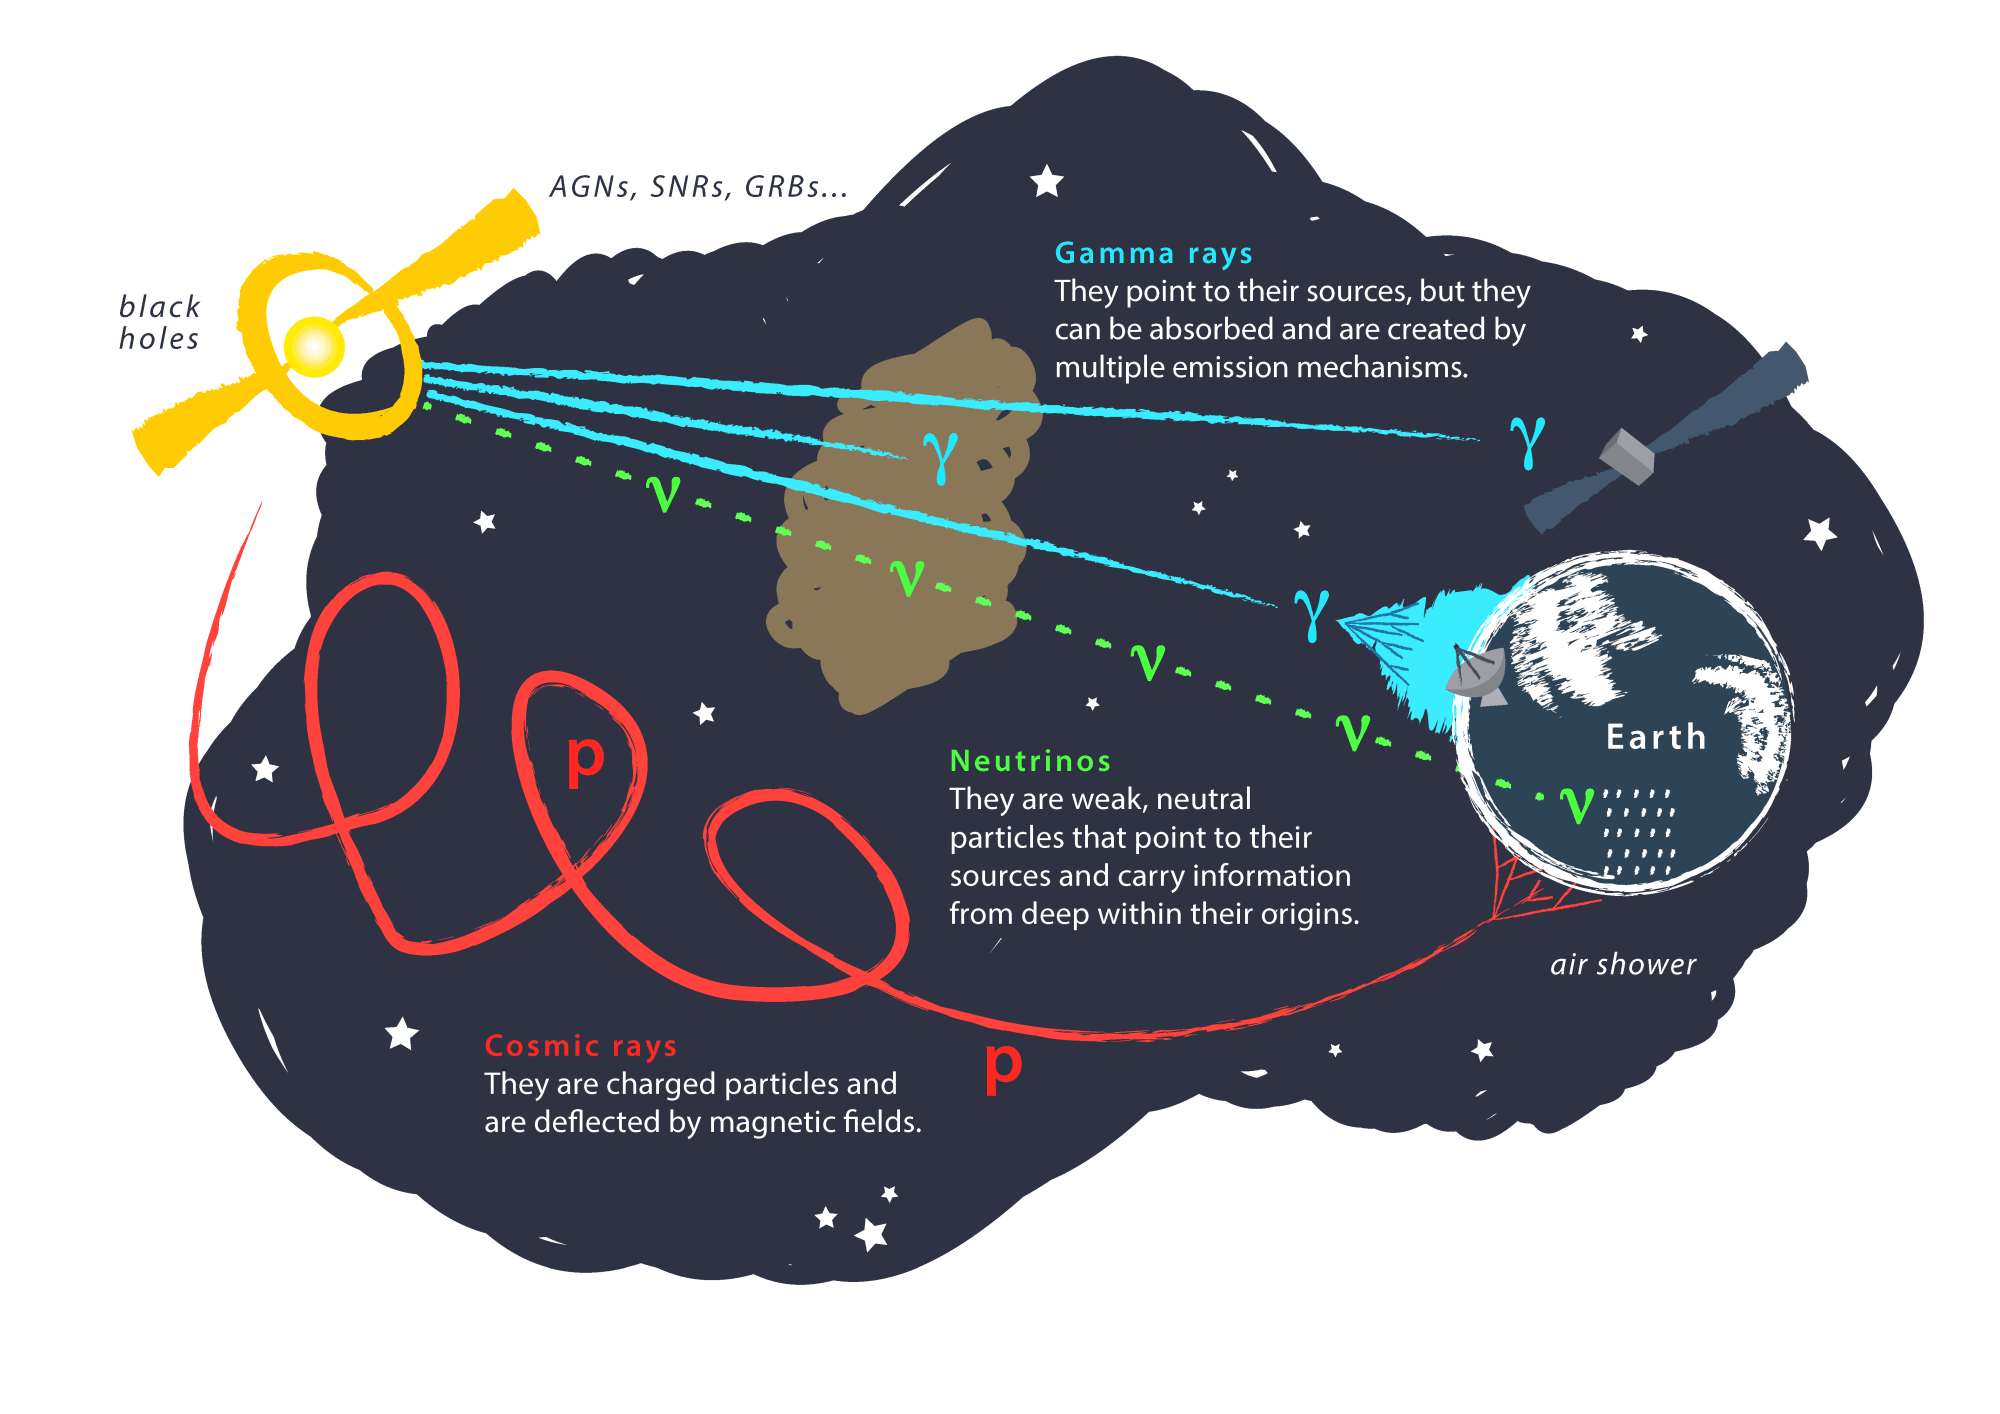
\includegraphics[width=0.8\textwidth]{graphics/figure5.png}
    \caption{Different types of cosmic messengers on their way to Earth. Charged particles like protons and electrons
    are deflected by magnetic fields and therefore making it hard to pinpoint the source. Only the
    origin of photons and neutrinos can be reconstructed directly since they are uncharged particles
    and therefore travel in straight lines. However, photons can be absorbed or created in multiple
    mechanisms. Since neutrinos only rarely interact with matter via the weak force, their detection
    is significantly harder than for photons \cite{fig5}.}
    \label{fig:fig5}
\end{figure}

Only \(\num{50}\) years after Hess' discovery, in 1961, Explorer XI \cite{explorer11}, the first satellite experiment
to measure gamma rays from space was launched, providing measurements of gamma rays above
\SI{50}{\mega\eV}, thus starting gamma-ray astronomy from space-based experiments. Just a few years
earlier neutrinos were already discovered by Cowan and Reines \cite{cowan1956}, with solar neutrinos being
discovered by Davis \etal{} \cite{davis} in the 1960s at the Homestake experiment.
The first detection of neutrinos from a supernova was made by the Kamiokande experiment in 1987
\cite{kamiokande1987}. The most recent discovery of a cosmic messenger has been that of gravitational
waves in 2015 \cite{grav_waves}.

Cosmic messengers come in different types, that are either charged or uncharged, as shown in \autoref{fig:fig5}.
\gls{cr} like electrons, protons or atomic nuclei are charged particles making it difficult to trace back their origin
as they are deflected by the cosmic electromagnetic fields. Uncharged particles like photons or
neutrinos, however, travel in straight lines, making it easier to reconstruct their origins.

While photons can be absorbed by dust clouds on their way to Earth, they are easier to detect than
neutrinos, the latter interacting only weakly with matter due to their small cross-section.
This means that neutrino detectors and experiments, such as IceCube \cite{icecube_2006} or
Super-Kamiokande \cite{kamiokande}, have to be large enough to detect the neutrinos in sufficient quantities.

In recent years, gamma-ray astronomy has become an important research field in astroparticle physics.
The term gamma-rays is generally denoted as photons with energies above \SI{100}{\kilo\eV}
\cite{funk}. Due to this high-energy nature, gamma rays pose some of the most powerful \gls{cr} in
the universe and since photons at such energies cannot be produced by thermal processes, their origin
can be described by higher order processes involving charged particles.

\begin{figure}
    \centering
    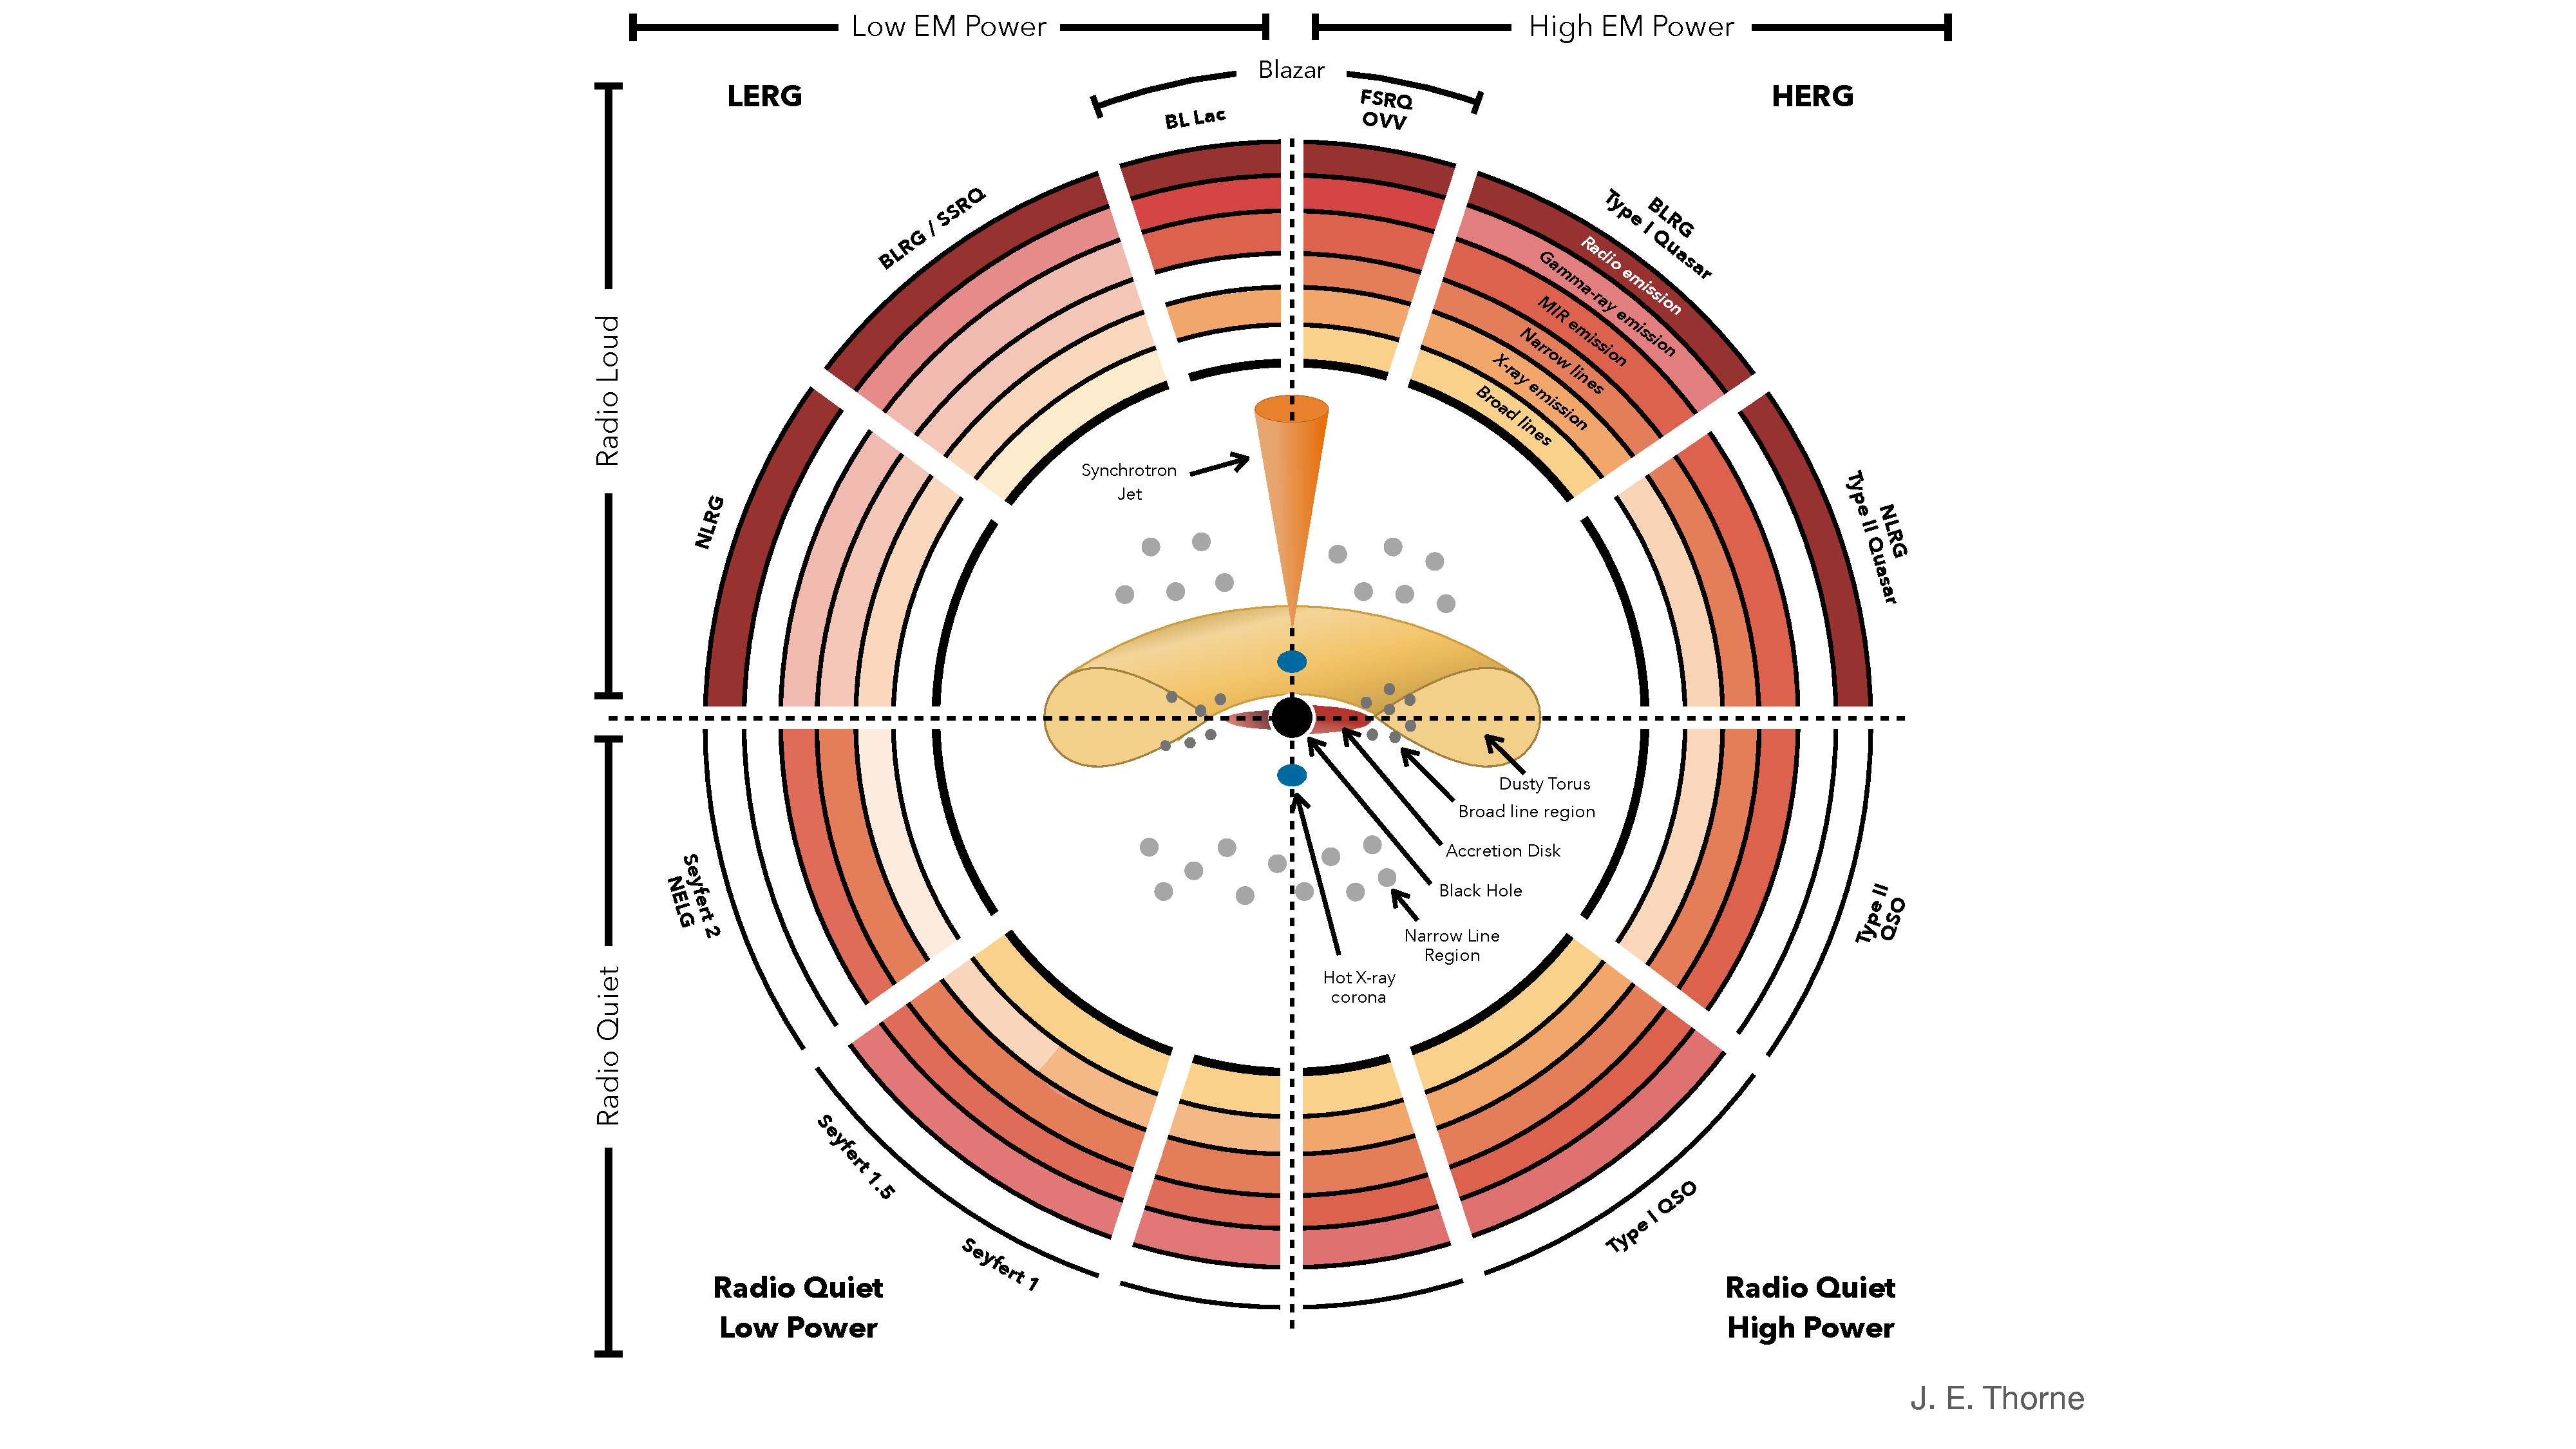
\includegraphics[width=\textwidth]{graphics/agn.pdf}
    \caption{Unified \gls{agn} model showing the different classifications for \glspl{agn}.
    An \gls{agn} is classified by the existence of a relativistic jet, the viewing angle of the observer
    or how bright it is \cite{agn_diagram}.}
    \label{fig:agn}
\end{figure}

Some of the brightest sources of gamma rays in our galaxy are \glspl{snr} such as the Crab Nebular.
The Crab Nebula, in particular, poses as a so-called standard candle with its constant flux of
\gls{hegr}, allowing to test the performance of new experiments and telescopes. Other sources for
gamma rays include \glspl{grb}, Pulsars and \glspl{agn}, the latter being one of the most common types
of extragalactic gamma-ray sources. \glspl{agn} accrete dust and matter in an accretion disk around the
central black hole. The matter gets accelerated by the gravitational force of the black hole and heats
up. While the exact process is not yet fully understood, some accretion disks form a relativistic jet
which, aside from other wavebands, also emits gamma rays via synchrotron
and inverse-Compton scattering processes. \glspl{agn} themselves can be classified depending on the existence
of a relativistic jet, the viewing angle of the observer or how bright they are. \autoref{fig:agn}
shows the different classifications of \glspl{agn}.

Gamma rays can be detected by a variety of experiments, either ground- or space-based. Space-based
experiments like the \gls{fermilat} are usually more sensitive to lower energies, but their performance
is lower for higher energies, as their effective collection area is comparatively small. Ground-based
experiments, however, are more sensitive to higher energies, although they have to rely on the scattering
of secondary particles in \glspl{eas} induced by the primary particle in Earth's atmosphere.
\autoref{fig:fermilat} shows the gamma-ray sky as observed by the \gls{fermilat} over a span of
\(\num{12}\) years.

\begin{figure}
    \centering
    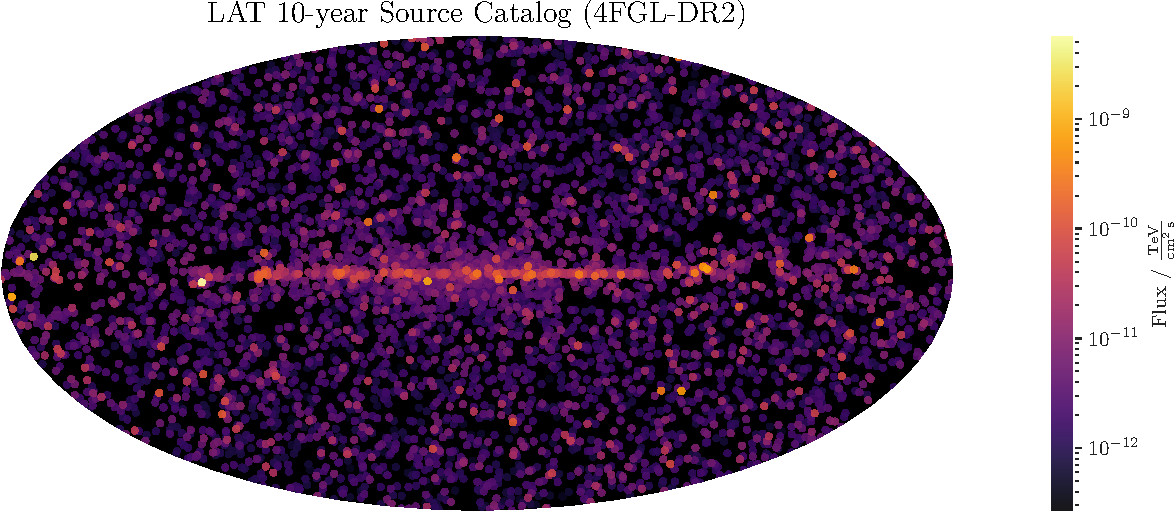
\includegraphics[width=0.8\textwidth]{build/fermi_catalog.pdf}
    \caption{Mollweide projection of the \gls{fermilat} 4FGL-DR3 catalog data of gamma-ray sources. The sky map
    shows the flux of gamma-ray sources in \(\si{\tera\eV\per\centi\meter\squared\per\second}\)
    observed over a span of \(\num{12}\) years from the experiment's launch in 2008. Additionally,
    the Crab Nebula (red circle) is marked along with \glspl{snr} (green circles) and \glspl{agn} (blue circles) that \gls{fermilat}
    observed \cite{fermi4fgl, fermi4fgldr3}. \todo[inline]{think about this remark -> keep AGNs? Also, use correct colors}Note that the marked \glspl{agn} are non-blazar active galaxies, that were
    selected because they represent extragalactic sources of gamma rays without blocking too much of the plot.}
    \label{fig:fermilat}
\end{figure}

For the past two decades, ground-based \gls{iact} experiments like the \gls{magic} telescopes, the
\gls{veritas} and the \gls{hess} have been monitoring these \gls{vhegr} to gain an understanding of
their production. This allowed us to determine different source classes inside and outside our galaxy,
with the most important source class inside our galaxy being \glspl{snr} such as the Crab Nebula.






\chapter{IACTs and the Cherenkov Telescope Array}
\glsreset{iact}

Modern gamma-ray observations are performed with either space-based experiments or with
ground-based experiments like water Cherenkov tanks such as the \gls{hawc} \cite{hawc} experiment or \glspl{iact}, the latter
being telescopes that use the Cherenkov light emitted by \glspl{eas} in the atmosphere.
In the following sections, I will introduce \glspl{iact} and the \gls{cta} and explain the mechanisms
that make it possible to observe gamma rays with these types of experiments.


\section{Imaging Air Cherenkov Telescopes}
\label{sec:iact}

Because of their ground-based setup, \glspl{iact} are taking advantage of the Earth's atmosphere to get a
larger effective area than any space-based instrument. This is especially helpful for energies above
\SI{100}{\giga\eV},
\begin{wrapfigure}[24]{r}{0.48\textwidth}
    \centering
    \vspace*{-0.5cm}
    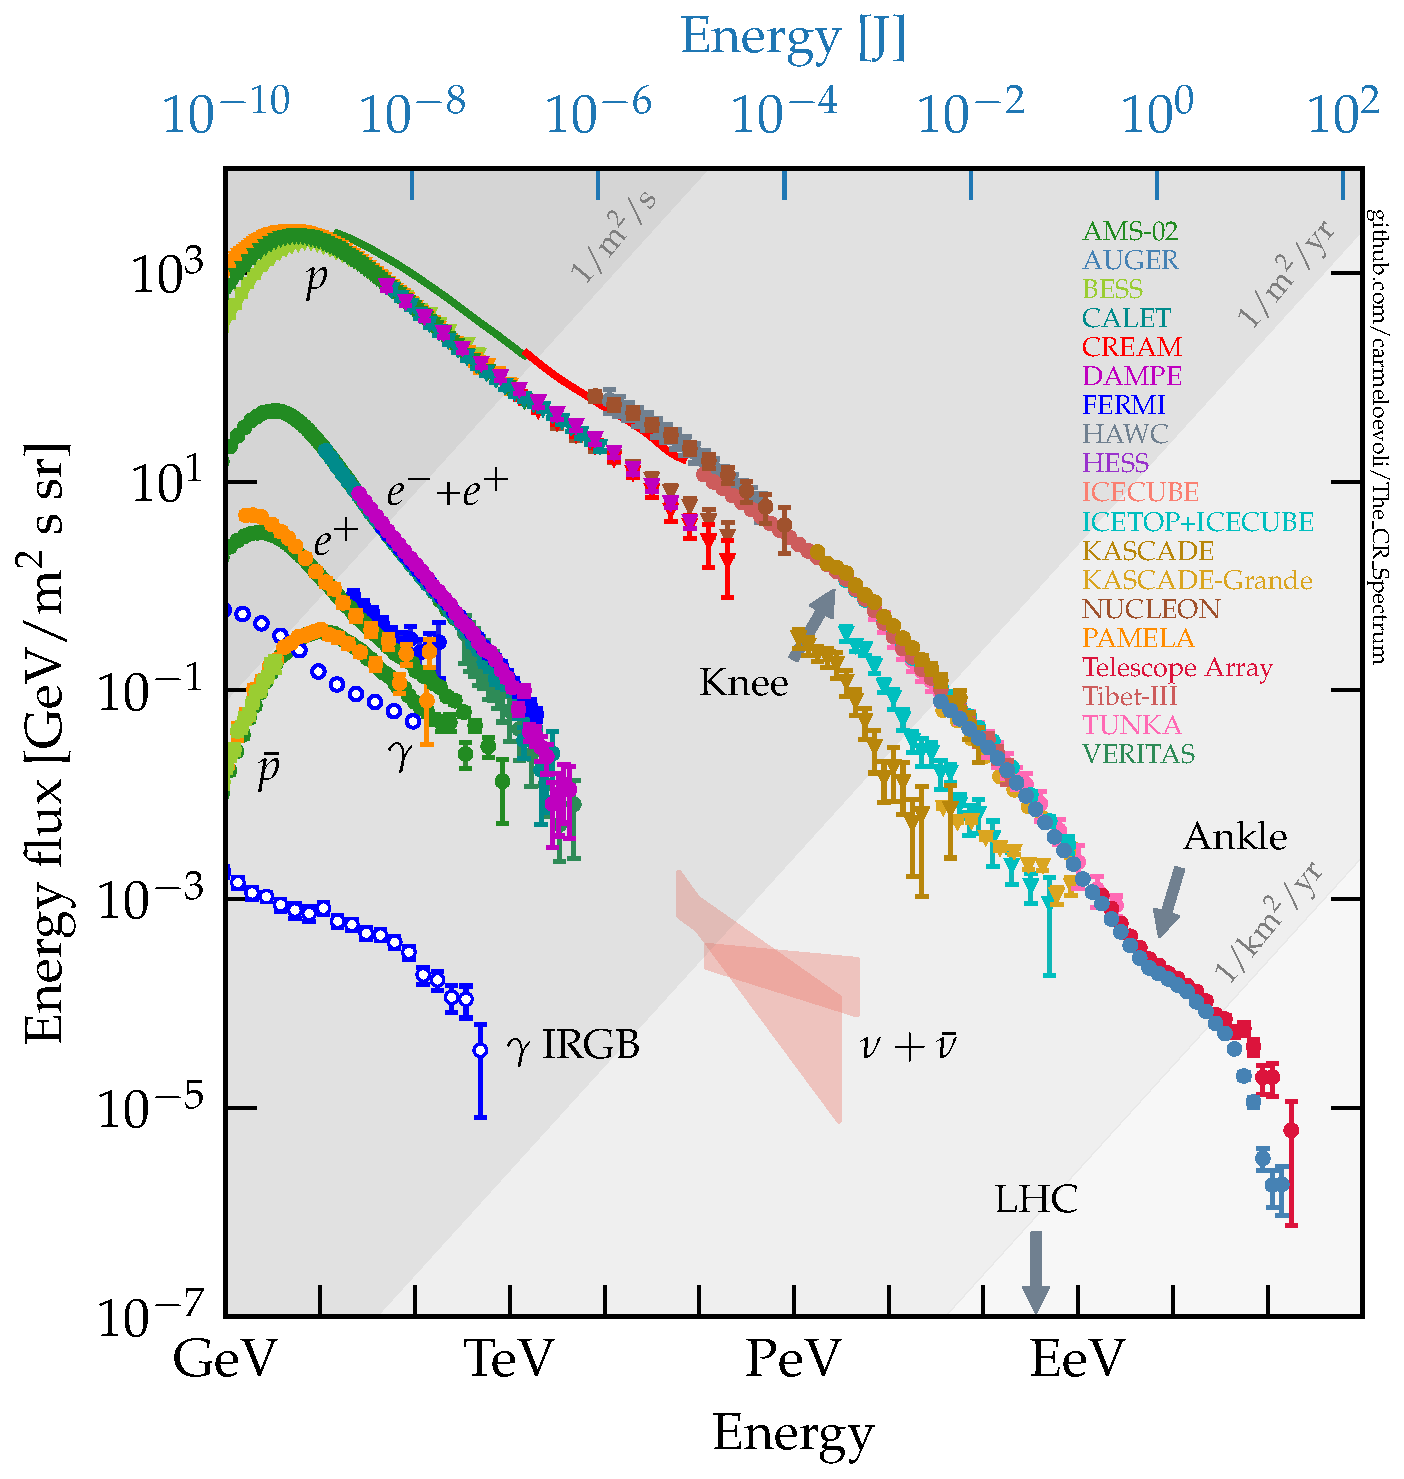
\includegraphics[width=0.46\textwidth]{graphics/cr_spectrum.pdf}
    \caption{The cosmic ray flux as a function of energy. For very high energies the flux becomes very
    small with only \(\num{1}\) particle per square meter per year reaching Earth. For even higher
    energies in the domain of \si{\exa\eV} this flux becomes \(\num{1}\) particle per square
    kilometer per year \cite{carmelo_2020}.}
    \label{fig:flux}
\end{wrapfigure}
where the gamma-ray flux is low, whereas lower energies show higher fluxes. At such high energies,
space-based instruments, experiments such as \gls{fermilat}, see fewer high-energy events compared
to ground-based experiments, due to their comparatively small effective collection area \cite[p.~256]{funk}.
The cosmic ray flux in \autoref{fig:flux} shows this well: The flux decreases rapidly with higher
energies, with only one high-energy (\greater\(\SI{40}{\giga\eV}\)) photon per day and square meter
reaching Earth from the Crab Nebula \cite{noethe_thesis} and even fewer photons for energies in the
\si{\exa\eV} domain, where only \(\num{1}\) particle per square kilometer per year reaches Earth.

Earth's atmosphere is opaque to \gls{he} gamma rays, so ground-based experiments rely on
cascades of sub-particles in so-called \glspl{eas}. For gamma-ray astronomy, the electromagnetic
component of these \glspl{eas}, shown in \autoref{fig:heitler_model}, is of interest, as these
are produced by gamma rays. When a gamma ray interacts with Earth's atmosphere, it decays into an
electron and a positron via pair production. These charged particles then emit more photons via
bremsstrahlung. These photons, again, produce more charged particles, which in turn emit even more
photons. This process continues until any of these processes reaches energies below a certain
threshold, \ie \SI{1022}{\kilo\eV} for the pair production process. For these processes to happen,
the particles have to be in the fields of the atoms of the Earth's atmosphere. As the particles
travel at speeds faster than light in the atmosphere, they emit Cherenkov light at
a fixed angle \(\theta\) with respect to the refraction index \(n\) of the atmosphere and the
factor \(\beta = \sfrac{v}{\symup{c}}\). The angle can be determined trigonometrically as
\begin{equation}
    \cos\theta = \frac{1}{\beta n},
\end{equation}
as can be seen in \autoref{fig:cherenkov}.

\begin{figure}
    \begin{subfigure}[t]{0.45\textwidth}
        \centering
        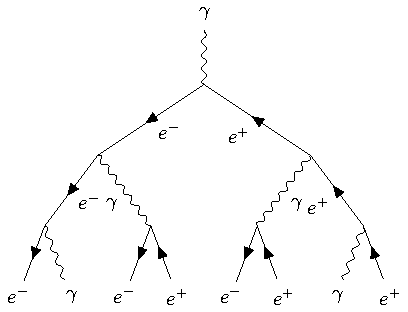
\includegraphics[width=0.90\textwidth]{graphics/heitler_model.pdf}
        \caption{Simplified first steps of the Heitler model of the electromagnetic component of an extensive air shower.
        A gamma ray induces an electron and a positron via pair production that then emit more photons
        via bremsstrahlung.}
        \label{fig:heitler_model}
    \end{subfigure}
    \hfill
    \begin{subfigure}[t]{0.45\textwidth}
        \centering
        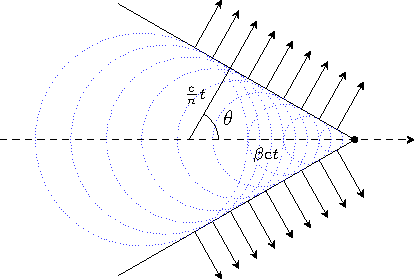
\includegraphics[width=0.90\textwidth]{graphics/cherenkov_radiation.pdf}
        \caption{Cherenkov radiation (outward-pointing arrows) from a charged particle traveling at
        uniform velocity, faster than the speed of light in the medium. The dashed line shows the
        path of the particle over time.}
        \label{fig:cherenkov}
    \end{subfigure}
    \caption{The electromagnetic component of an extensive air shower (see \hyperref[fig:heitler_model]{(a)})
    is induced by gamma rays that then decay into electrons and positrons via pair production.
    These charged particles will emit more gammas via bremsstrahlung, which again will produce
    new electrons and positrons. This will continue until the energy of the gammas is below
    the threshold of \SI{1022}{\kilo\eV} for pair production. Another process is the production of
    Cherenkov light from the electrons and positrons, which is shown in \hyperref[fig:cherenkov]{(b)}.
    The Cherenkov light is the result of the charged particles traveling faster than the speed of light
    in the atmosphere, thus emitting photons in a fixed angle \(\theta\) \wrt the refraction index
    \(n\) of the medium and the factor \(\beta\).}
    \label{fig:cherenkov_heitler}
\end{figure}

Cherenkov light emitted by \glspl{eas} can then be collected by an IACT's mirrors and detected by
its camera within a timeframe of an order of nanoseconds. The resulting image will show the shape
of the air shower and can be used to determine the shower's primary particles' properties and
reconstruct its origin. As the hadronic component of \glspl{eas} produce
electromagnetic subshowers, \glspl{iact} have a dominant hadronic background, which has to be
separated from the gamma ray-induced showers, for example with
machine learning algorithms. Before this separation, however, signal pixels in the camera image have
separated from the electronic noise coming from the camera as well as from the \gls{nsb} with the help of
cleaning algorithms. This will be the focus of this work. These cleaning algorithms pose a vital step
in the analysis of an event, as only a fraction of all pixels in the camera frame are part of the signal.


\section{The Cherenkov Telescope Array}
\label{sec:cta}

\cta{} is a new generation of \glspl{iact} that will consist of two sites,
one of which will be built at the \gls{orm} on the Canarian island of La Palma while the other one
will be built in the southern hemisphere at the \glspl{eso} Paranal Observatory in the Atacama desert
of northern Chile.

\cta{} consists of three types of telescopes, shown in \autoref{fig:cta_telescopes}, each being
sensitive to a different energy range \cite{cta_specs}:
\begin{description}
    \item [] \textbf{\gls{lst}}: The largest telescopes in \cta{} have a primary deflector diameter
    of \SI{23}{\meter} with a field of view of \SI{4.3}{\deg} and provide full system sensitivity in the energy
    regime from \(\SI{20}{\giga\eV}\) to \(\SI{150}{\giga\eV}\).
    \item [] \textbf{\gls{mst}}: The \glspl{mst} have a primary deflector diameter of \SI{11.5}{\meter}
    with a field of view of \SI{7.7}{\deg} for their NectarCam and provide full system sensitivity in the energy
    regime from \(\SI{150}{\giga\eV}\) to \(\SI{5}{\tera\eV}\).
    \item [] \textbf{\gls{sst}}: Being the smallest telescope type in \cta{}, the \glspl{sst}
    have a primary deflector diameter of \SI{4.3}{\meter}, a secondary deflector diameter of
    \SI{1.8}{\meter} with a field of view of \SI{10.5}{\deg} and provide full system sensitivity in the energy
    regime from \(\SI{5}{\tera\eV}\) to \(\SI{300}{\tera\eV}\).
\end{description}

\begin{figure}
    \centering
    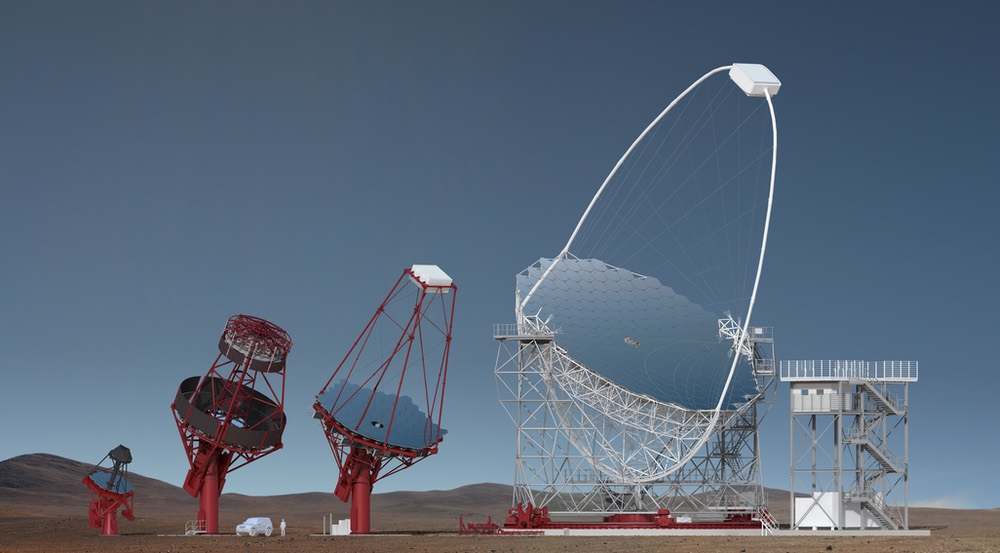
\includegraphics[width=0.7\textwidth]{graphics/telescopes_render.jpg}
    \caption{A rendered image of the 3 telescope prototypes in \cta{}. From left to right: The \gls{sst},
    two types of \gls{mst} (SCT and MST) and the \gls{lst}. This work will not feature the SCT, as
    the simulation data used contains only \gls{lst} and \gls{mst} data for the northern array.
    Image credit: Gabriel Pérez Diaz, IAC \cite{cta_tech}.}
    \label{fig:cta_telescopes}
\end{figure}

Since the southern hemisphere has a better view of the galactic center than the northern hemisphere,
only \cta{} south will feature the \glspl{sst} along the other two telescope types. \cta{} north
will only feature \glspl{mst} and \glspl{lst}. In its full configuration, \cta{} would feature
\(\num{70}\) \glspl{sst}, \(\num{25}\) \glspl{mst} and \(\num{4}\) \glspl{lst} at \cta{} south,
and \(\num{15}\) \glspl{mst} and \(\num{4}\) \glspl{lst} at \cta{} north. However, the reduced
layout---called Alpha Configuration---is the currently planned layout for both \cta{}
north and south. This work will focus on the northern site, consisting of \(\num{9}\) \glspl{mst}
and \(\num{4}\) \glspl{lst} \cite{cta_north_layout}. \autoref{fig:cta_layout} shows the planned
Alpha Configuration layout of both sites of \cta{} where \cta{} south is displayed with its
\(\num{37}\) \glspl{sst}, \(\num{14}\) \glspl{mst} and the \(\num{4}\) \glspl{lst} in the center
\cite{cta_south_layout}.
\begin{figure}
    \centering
    % \includegraphics[width=0.75\textwidth]{graphics/cta_alpha_layout.pdf}
    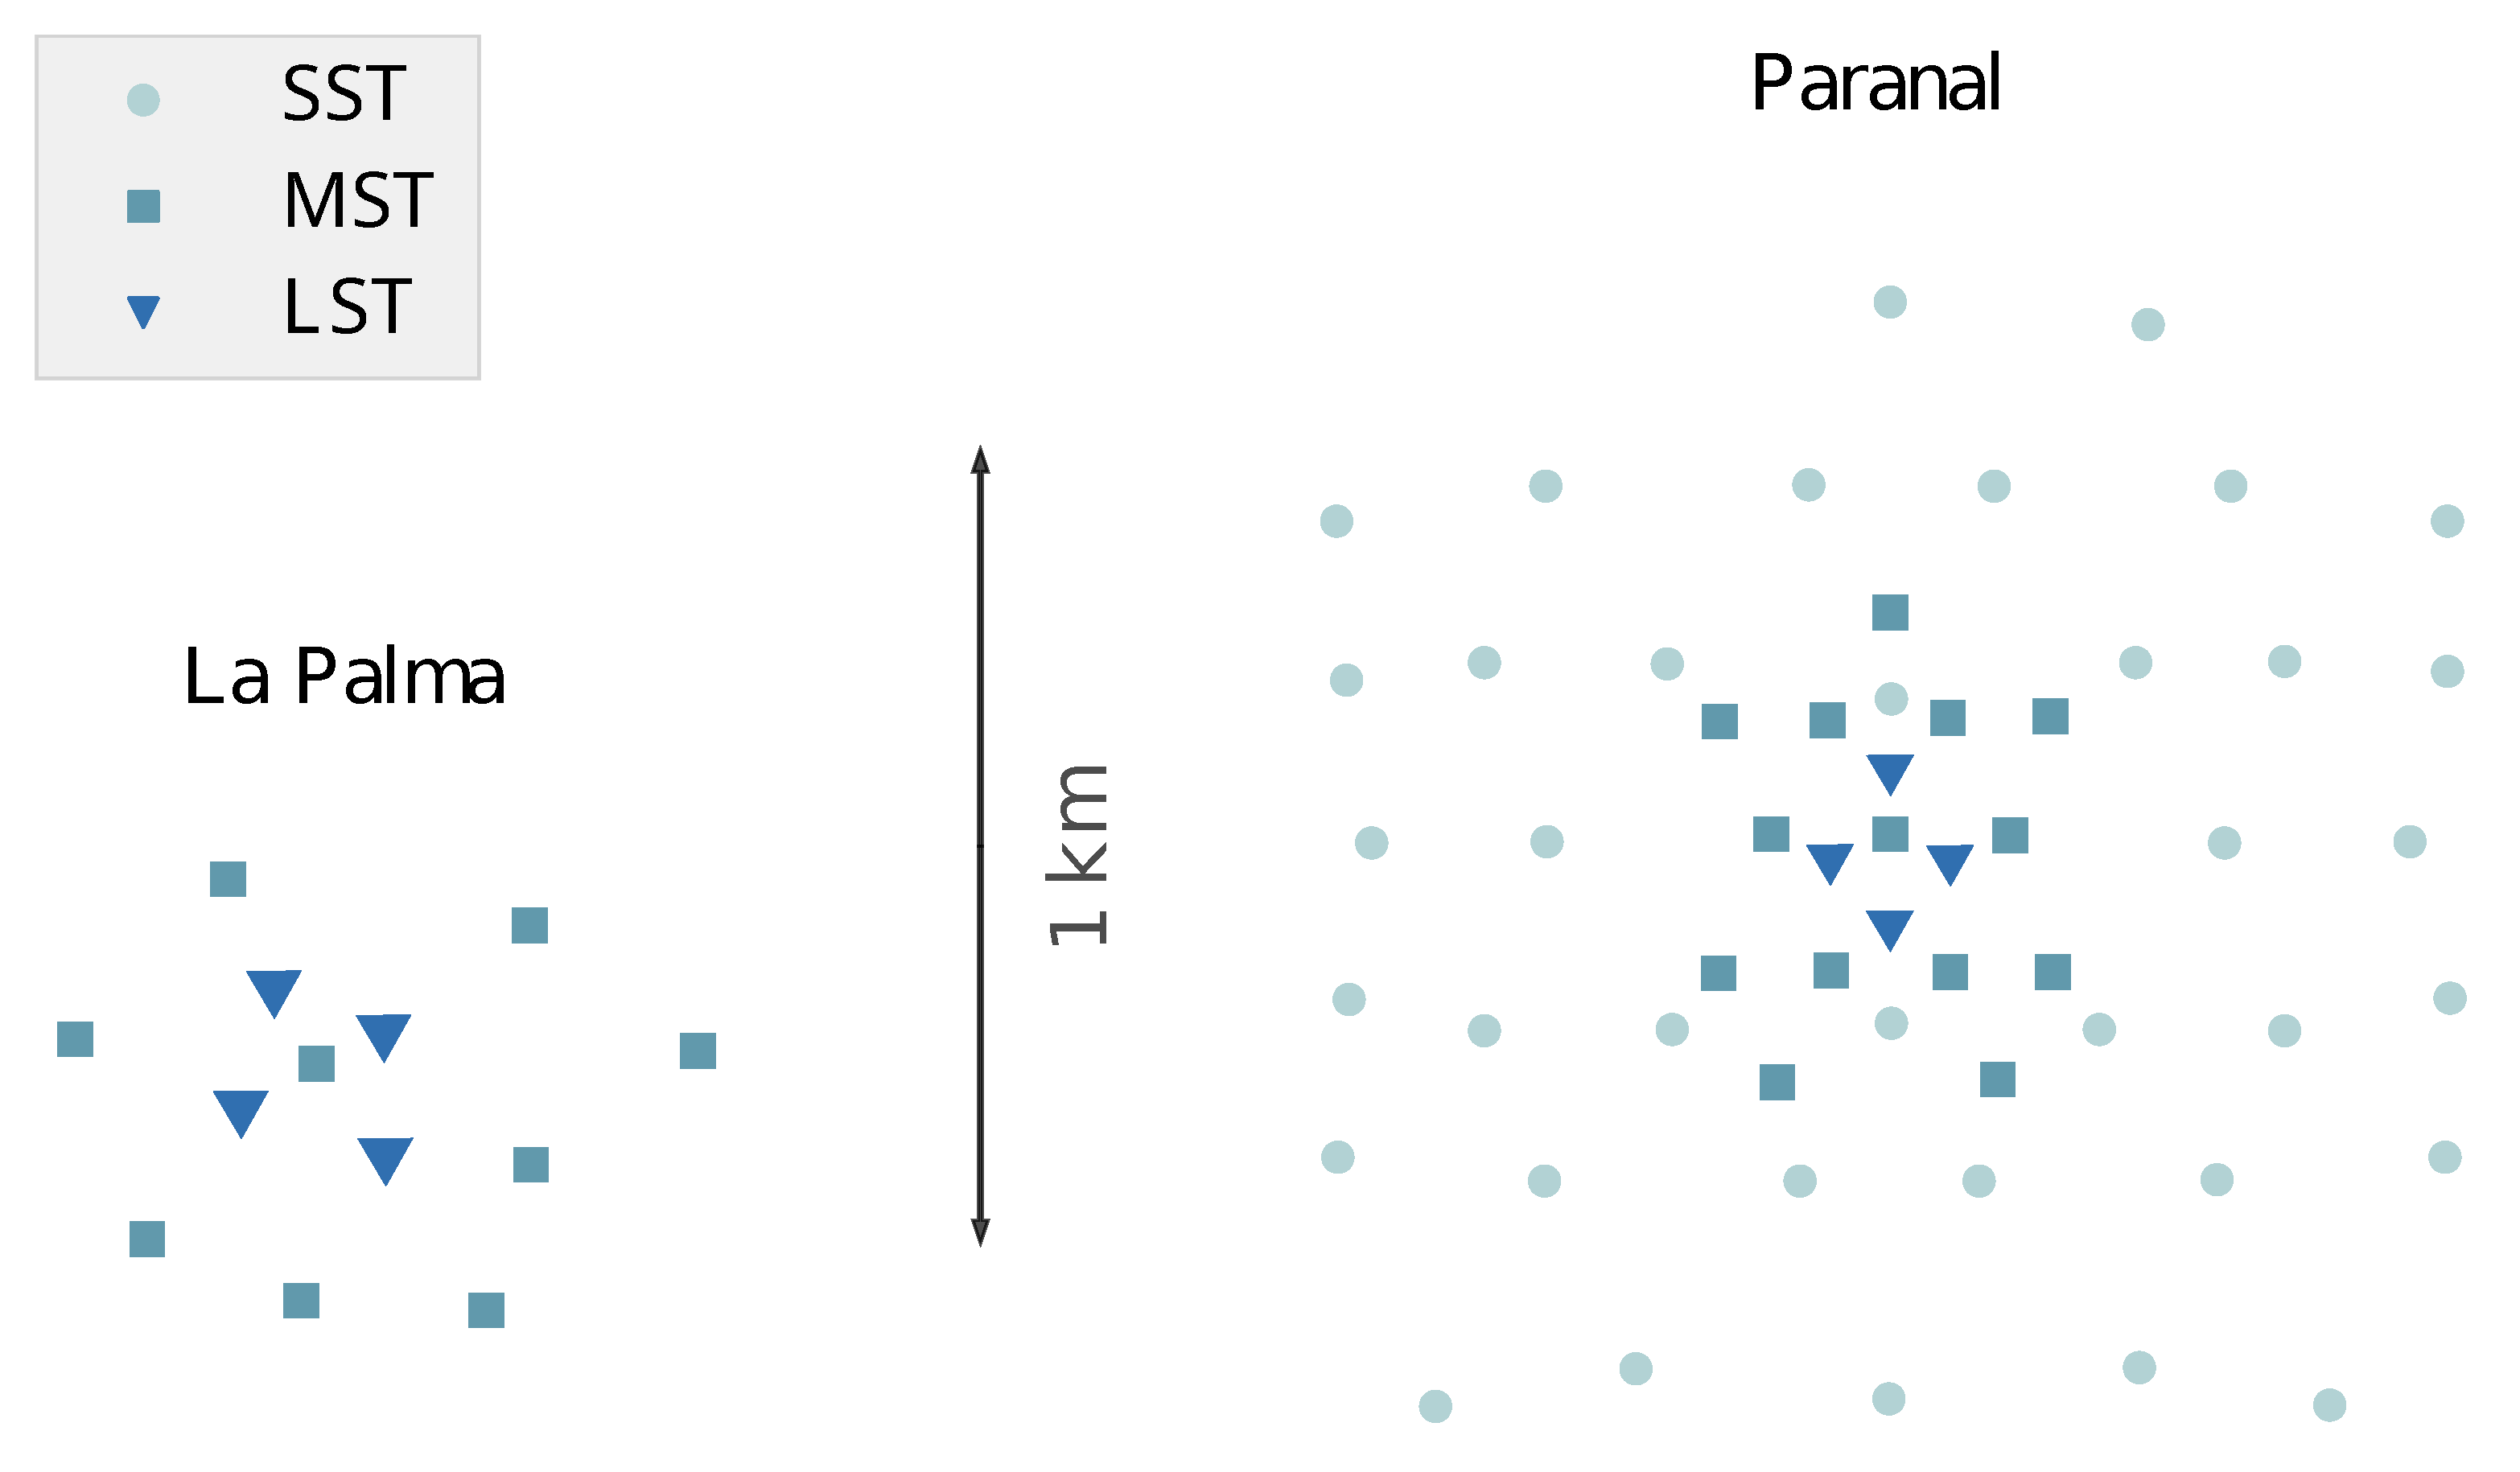
\includegraphics[width=0.75\textwidth]{graphics/cta_layout.pdf}
    \caption{Alpha Configuration layout of the \cta{} north and \cta{}
    south site. \cta{} south would feature \(\num{37}\) \glspl{sst}, \(\num{14}\) \glspl{mst} and
    \(\num{4}\) \glspl{lst} \cite{cta_south_layout} in it's Alpha Configuration, while \cta{} north would
    feature \(\num{9}\) \glspl{mst} and \(\num{4}\) \glspl{lst} \cite{cta_north_layout}.
    This figure was adapted from Kai Br\"ugge in his Ph.D. thesis \cite{bruegge_thesis}.}
    \label{fig:cta_layout}
\end{figure}

The \gls{mst}'s and \gls{lst}'s cameras are based on \gls{pmt} photodetectors, while the \gls{sst}'s
camera is based on a \gls{sipm} photodetector. Both detector types provide fast response times in the
order of nanoseconds. \glspl{pmt} can detect small amounts of electromagnetic radiation due to their
amplification process. However, this amplification process also amplifies the noise of the detector
and needs higher voltages than \glspl{sipm}. The latter, on the other hand, needs to be cooled,
as \glspl{sipm} are prone to having a higher dark current at higher temperatures.
% The \gls{mst} and \gls{lst} will feature a camera with \(\num{1855}\) pixels.

With \cta{} probing the \gls{vhe} gamma-ray sky and a resolution outperforming predecessors, like
\gls{hess} or \gls{magic}, it will be able to observe a broad variety of sources, allowing insights
into interaction processes of \gls{vhegr} as well as their origin.

Together with gravitational wave and neutrino observatories as well as with other gamma observatories,
\cta{} will probe the universe in its \glsreset{he}\gls{he} domain, allowing to study a broad field of key questions
in astrophysics. As such, \cta's scientific goals can be divided into three categories \cite{cta_scientific_goals}:
\begin{description}
    \item [Origin and Role of relativistic Cosmic Particles:] \cta{} will try to find the sources of
    \gls{he} cosmic particle acceleration in the universe. This includes the search for the mechanisms
    that accelerate cosmic particles. Also, \cta{} will try to answer what role these particles play
    in feedback on star formation and galaxy evolution.
    \item [Extreme Environments:] \cta{} aims to deepen our understanding of the processes that
    are at work close to neutron stars and black holes, the characteristics of relativistic jets and
    \gls{pwn}. Also, it will probe the intensity of radiation fields and magnetic fields and how these
    would evolve over cosmic time scales.
    \item [Frontiers in Physics:] \cta{} will try to answer questions about the nature of dark matter
    and its distribution in the universe. As such, the existence of axion-like particles will be
    probed. Furthermore, \cta{} will search for quantum gravitational effects on photon propagation.
\end{description}


\chapter{Data processing with \ctapipe{}}
\label{ch:data-processing}

The analysis in this work was done with the open-source low-level data processing software for \cta{},
\ctapipe{} \cite{ctapipe}. The version used is the development version \texttt{0.15.1.dev166+gf26107f},
henceforth shortened to version \texttt{0.15.1}. The goal of \ctapipe{} is to provide a complete analysis
framework ranging from data calibration and image extraction to the reconstruction of events and the
analysis of their properties. In this chapter, I will first describe how the data
were simulated in \autoref{sec:data-simulation} and then, in \autoref{sec:data-levels}, explain the different
data levels and \ctapipe{}'s various analysis steps. In \autoref{sec:pipeline} I will
explain the full pipeline created for this work.


\section{Data simulation}
\label{sec:data-simulation}

In its current in-development state, \ctapipe{} is used and tested with simulated data, as the software
can only be sufficiently tested when the output is compared to truth data. This data is created with the help of
\gls{mc} simulations. The software used for these simulations is called \gls{corsika} \cite{corsika} and
allows for detailed simulation of \glspl{eas} initiated by \glspl{hecr}. The showers are observed by
a virtual \gls{iact} array, the \texttt{sim\_telarray} \cite{bernlohr2008}. The resulting so-called
\texttt{simtel} data is used in \ctapipe{} and can be processed as described in \autoref{sec:data-levels}
and \autoref{fig:ctapipe}. Some of the data properties are listed in \autoref{tab:simtel}.

This data is the basis for the analysis in this work. A total of
\(\num{20}\) \texttt{simtel} runs of diffuse gamma data were used for the initial analysis, \ie the
testing of different parameters as described in \autoref{sec:hyperparameters}. The individual runs
were processed into \dlo{} files and merged before being processed for each cleaning setting.

Once promising settings are found, a larger dataset containing \(\num{987}\) runs is processed with these
selected settings, allowing for more statistics and a better comparison of the cleaning algorithms.

\begin{table}
    \centering
    \caption{Simtel data properties of the \gls{corsika} simulation used for the datasets in this works
    analysis.}
    \label{tab:simtel}
    \rowcolors{0}{white!92!black}{}
    \begin{tabular}{l r}
        \hiderowcolors
        & Diffuse Gamma data \\
        \showrowcolors
        {Energy range / \si{\tera\eV}} & \numrange[range-phrase={--}]{0.003}{330} \\
        {Zenith angle / \si{\degree}} & \num{20} \\
        {View cone angle / \si{\degree}} & \num{10} \\
        {Number of showers} & \num{50000} \\
        {Spectral index} & \num{-2.0} \\
        {Maximum scatter range / \si{\meter}} & \num{1900} \\
    \end{tabular}
\end{table}


\section{Data Levels in \ctapipe{}}
\label{sec:data-levels}

There are several data levels in \ctapipe{}, spanning from the raw data \rzero{} to the reconstructed events
\dlt{}, with the raw data levels being denoted by an \textbf{R} and the calibrated data levels by a \textbf{D}.
\autoref{fig:ctapipe} shows a simplified overview of the data levels and the analysis steps.
The raw data level \rzero{} is the data that comes directly from the photodetectors. The time-resolved
signal of the data is calibrated from \rzero{} to \rone{}. Then the data volume gets reduced
(\rone{} \rightarrow \dlz{}) by a selection of waveforms.

The \dlz{} data level is the first level being stored and also the first level to be processed from
the simulation datasets used in this work. From \dlz{} to \dloa{}, the images of the data are extracted
from the time pulses, which are then cleaned by a cleaning algorithm, allowing for parametrization
of the events (\dloa{} \rightarrow \dlob{}). The parametrized events can then be reconstructed
(\dlob{} \rightarrow \dlt{}) and stored on the \dlt{} data level.

\begin{figure}
    \centering
    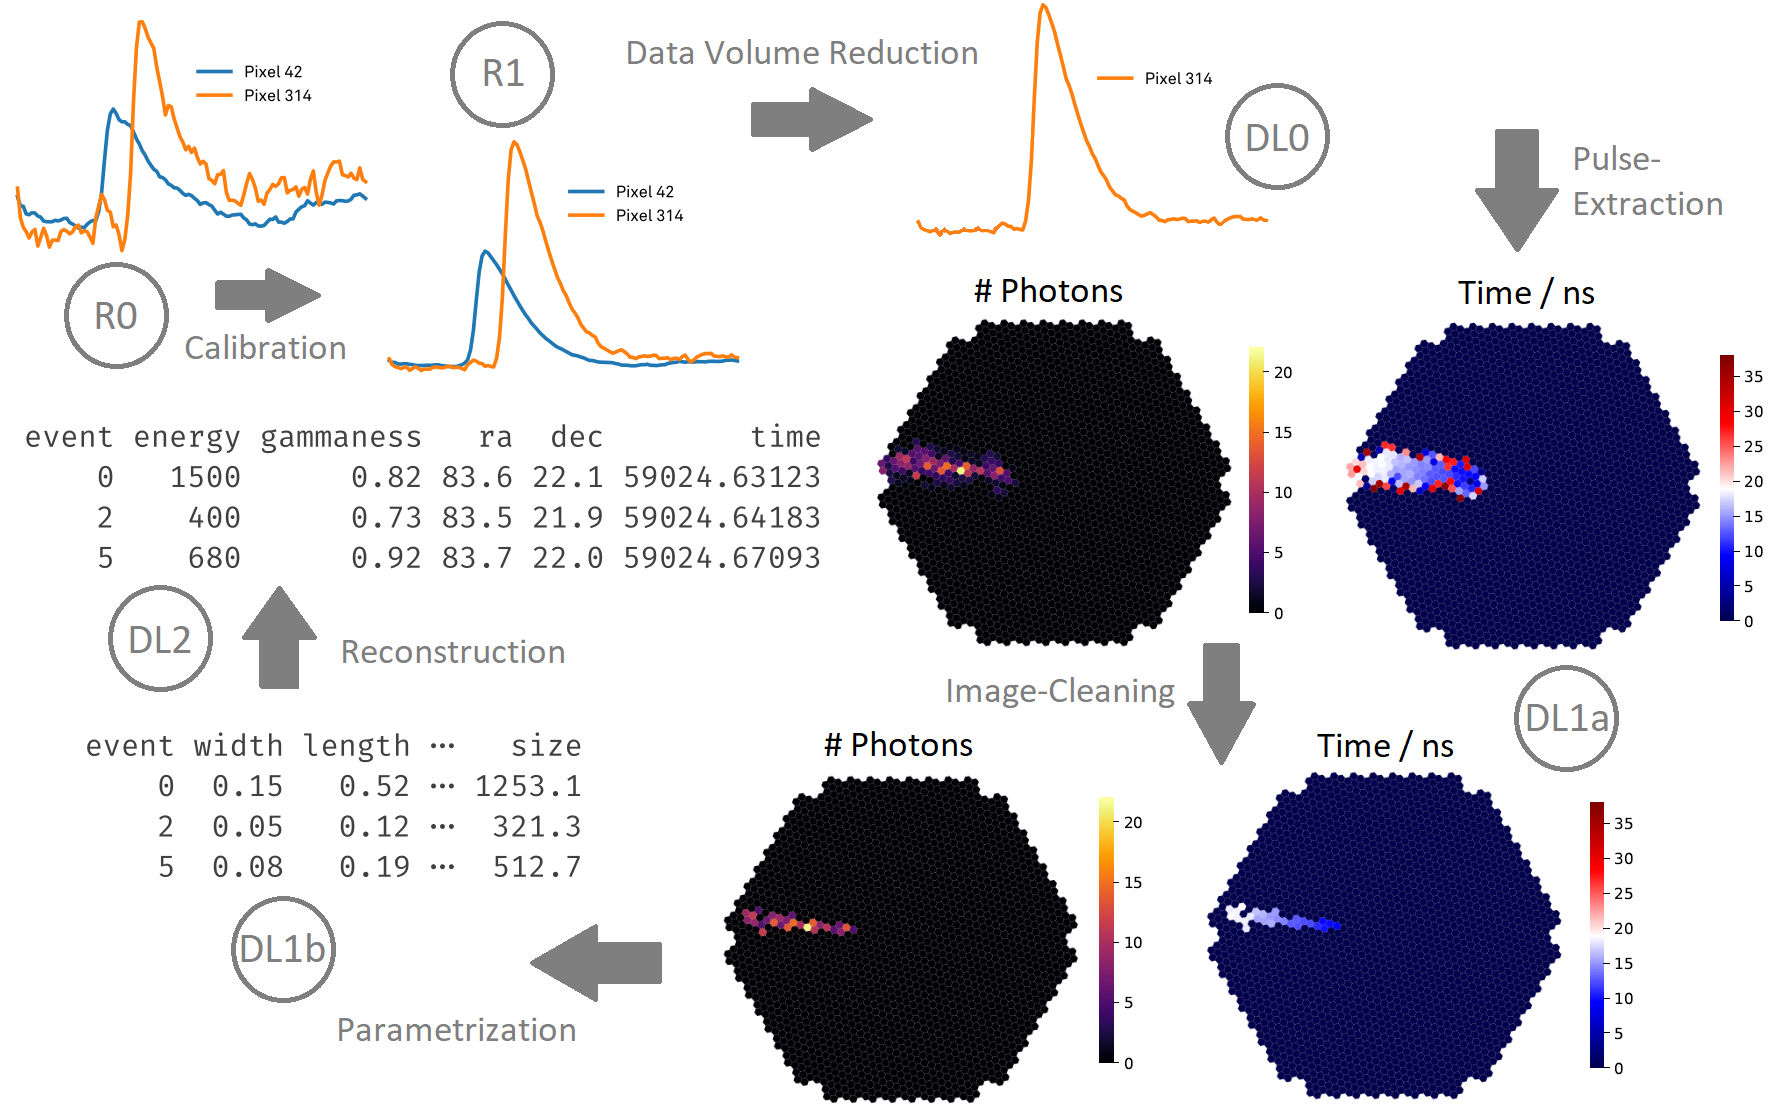
\includegraphics[width=\textwidth]{graphics/ctapipe.png}
    \caption{Data levels in \ctapipe{}. Raw data levels are denoted by an \textbf{R} and calibrated
    data levels by a \textbf{D}. The raw data first gets calibrated (\rzero{} \rightarrow \rone{})
    and then reduced in volume by selecting waveforms (\rone{} \rightarrow \dlz{}). From there the
    images are extracted (\dlz{} \rightarrow \dloa{}) and cleaned with a cleaning algorithm. This
    allows for parametrization of the events (\dloa{} \rightarrow \dlob{}). The parametrized events
    can then be reconstructed (\dlob{} \rightarrow \dlt{}) \cite{noethe_thesis, hackfeld}.}
    \label{fig:ctapipe}
\end{figure}

\section{This work's data processing pipeline}
\label{sec:pipeline}
In this work, the data processing pipeline is as follows: First, several simulation data runs are
selected and processed with \ctapipe{}. Then, the datasets are merged and serve as a basis for a re-run
of the combined dataset with various parameter combinations described in \autoref{ch:finding-hyperparams}.

The settings for \ctapipe{} are saved in two configuration files: First, a file, that sets up the
cleaning process and what data to write to the output file. For the preprocessing step of this work's
pipeline, the cleaning settings are not relevant, as this step only serves to create a merged dataset.
The second file contains a list of all the allowed telescope IDs. This allows a selection of the telescopes
that are used in the analysis. This is especially helpful if one wants to only analyze \gls{mst}-related
data, like in this work.

For the re-run of the combined dataset, the cleaning settings are used\footnote{As opposed to the preprocessing step},
however, as this step is the heart of this work's search for the optimal hyperparameters.
The configuration files used are shown in \hyperref[ap:config_files]{appendix \ref{ap:config_files}}.

Each resulting dataset can then be processed on an array or telescope data level, resulting in
\dloa{} image plots, values for the angular resolution and the efficiency as well as metrics for the
performance. An in-detail description of how this helps to compare the performance of the different
cleaning algorithms can be found in \autoref{sec:hyperparameters}. A schematic overview of the data
processing pipeline of this work is shown in \autoref{fig:data-processing}.

\begin{figure}
    \centering
    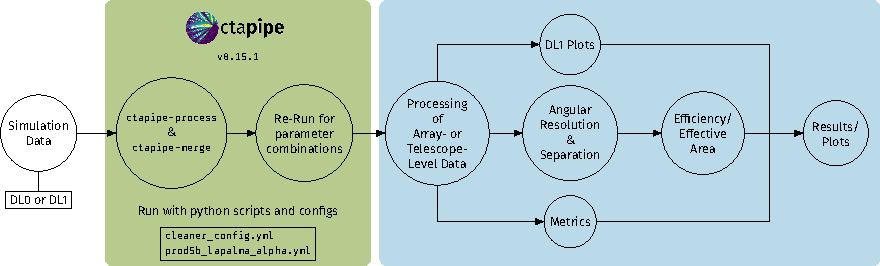
\includegraphics[width=\textwidth]{graphics/data_pipeline.pdf}
    \caption{Schematic overview of the data pipeline used for this work. Single runs of the simulation
    data are processed with \ctapipe\texttt{-process} and then merged via the tool \ctapipe\texttt{-merge} (green shaded area).
    The merged data is then processed on the array or telescope data level resulting in scores for metrics
    as well as \dlo{} \texttt{images} and plots for the angular resolution and the effective area (blue shaded area).}
    \label{fig:data-processing}
\end{figure}



\chapter{Finding Optimal Hyperparameters for the Cleaning Algorithms}
\label{ch:finding-hyperparams}

\section{Cleaning Algorithms}
\label{sec:cleaning-algorithms}

Version \texttt{0.15.1} of \ctapipe{} features four cleaning algorithms, two of which are time-based.
The \tailcuts{} algorithm is the most basic algorithm of the four and serves as a good
starting point for the development of new cleaning algorithms. Its first step is to select all
pixels that are above a certain threshold, the \texttt{picture} or \texttt{core\_threshold}. These
pixels are the core part of the signal and are the brightest. The \tailcuts{} algorithm
then selects all pixels that are above the so-called \texttt{boundary\_threshold} and are neighboring
the core pixels. A visualization of the algorithm is shown in \autoref{fig:tailcuts_clean} for the
default values of the algorithm.

\begin{figure}
    \centering
    \begin{subfigure}[t]{0.33\textwidth}
        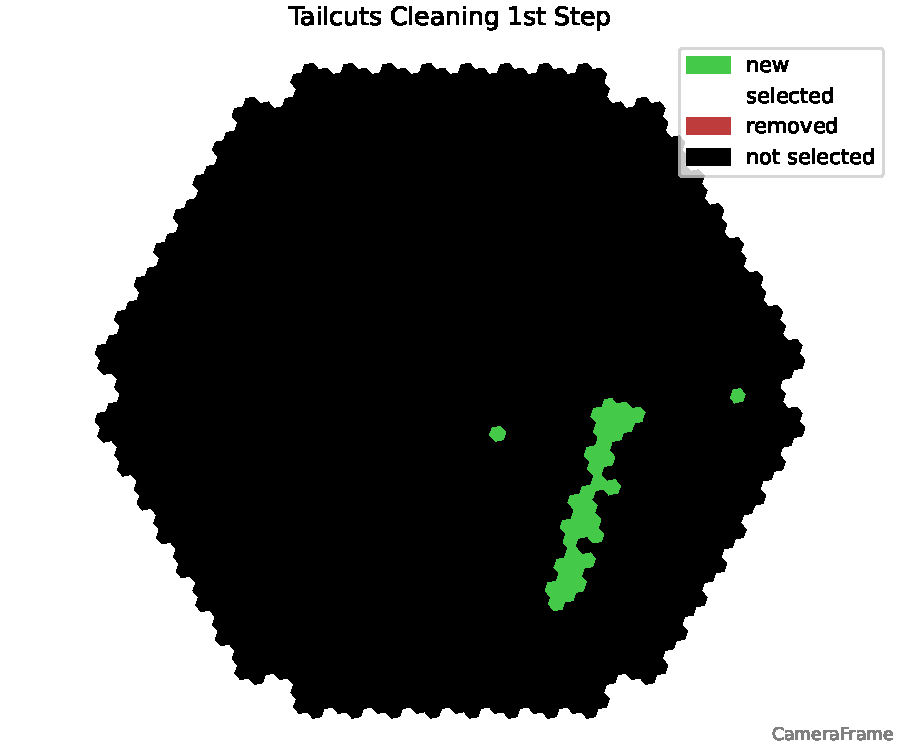
\includegraphics[width=\textwidth]{plots/cleaner_steps/tail_1.pdf}
    \end{subfigure}
    \begin{subfigure}[t]{0.33\textwidth}
        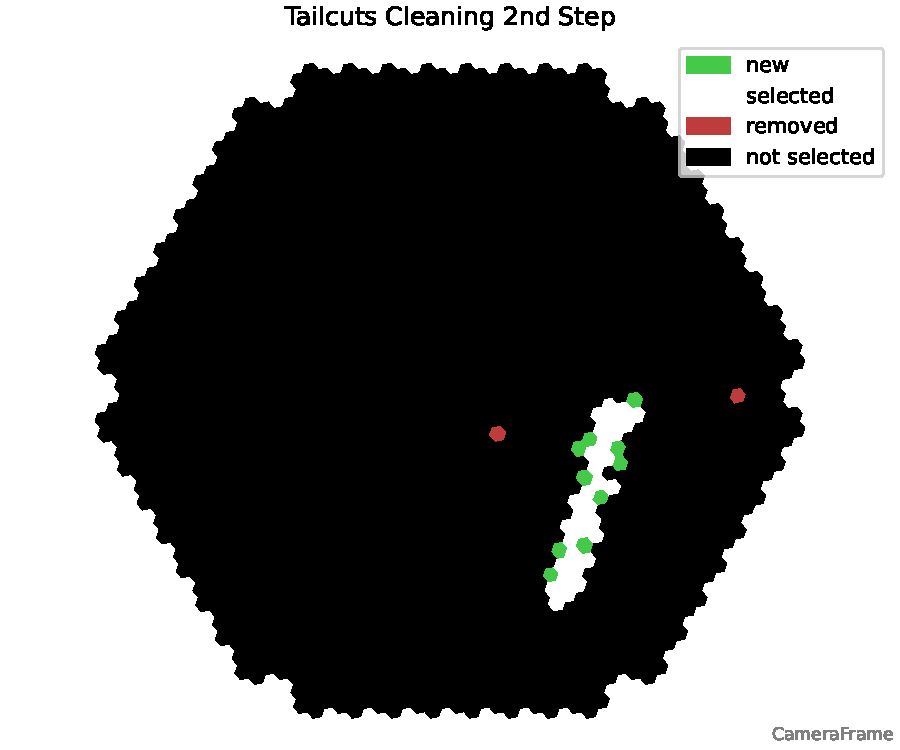
\includegraphics[width=\textwidth]{plots/cleaner_steps/tail_2.pdf}
    \end{subfigure}
    \caption{Visualization of the \tailcuts{} algorithm for a \gls{mst} NectarCam image. First, all
    pixels above the \texttt{core\_threshold} are selected. Then, all pixels neighboring the core
    pixels that are above the \texttt{boundary\_threshold} are selected.}
    \label{fig:tailcuts_clean}
\end{figure}

The \mars{} algorithm is very much based on the \tailcuts{}
algorithm and features an additional step, in that it also selects all neighbors of a neighbor of a
core pixel, if they are above the \texttt{boundary\_threshold}. The three steps for the \mars{} algorithm
are shown in \autoref{fig:mars_cleaning} for the default values of the algorithm.

\begin{figure}
    \centering
    \begin{subfigure}[t]{0.32\textwidth}
        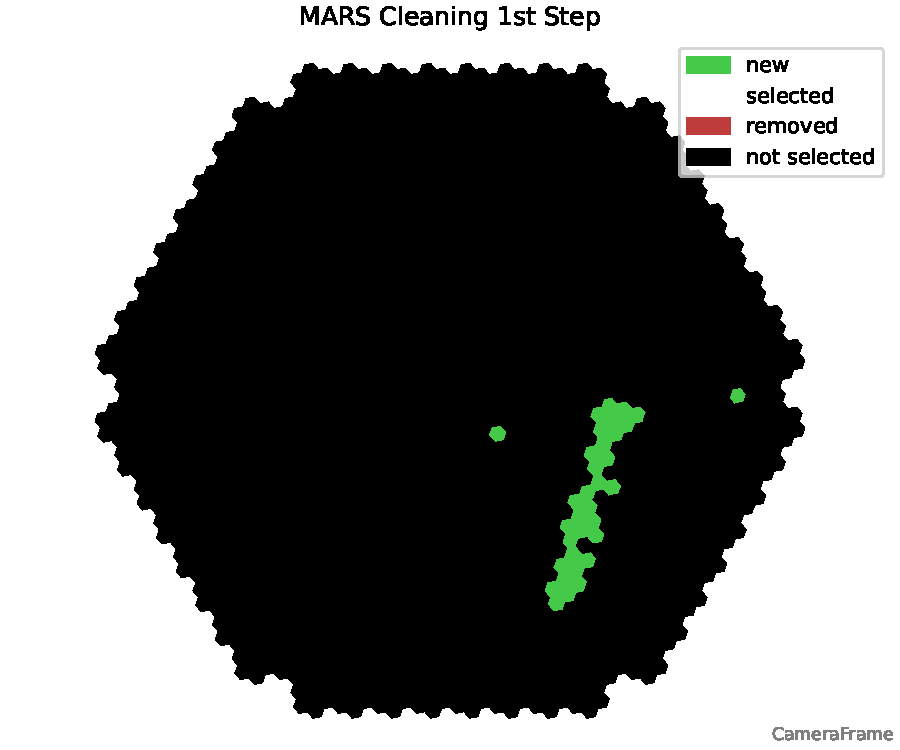
\includegraphics[width=\textwidth]{plots/cleaner_steps/mars_1.pdf}
    \end{subfigure}
    \hfill
    \begin{subfigure}[t]{0.32\textwidth}
        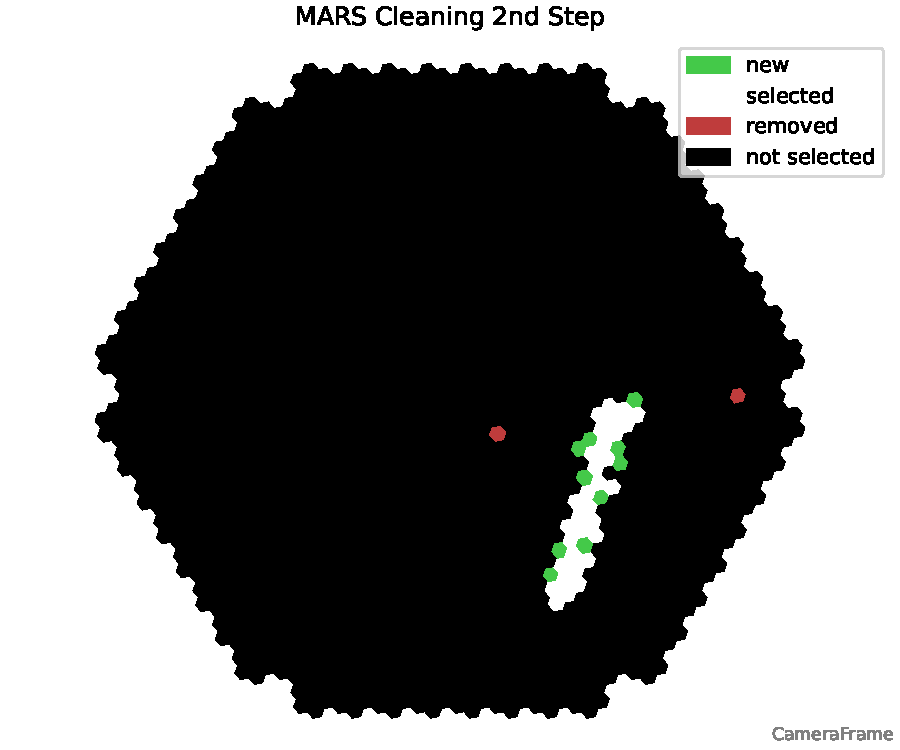
\includegraphics[width=\textwidth]{plots/cleaner_steps/mars_2.pdf}
    \end{subfigure}
    \hfill
    \begin{subfigure}[t]{0.32\textwidth}
        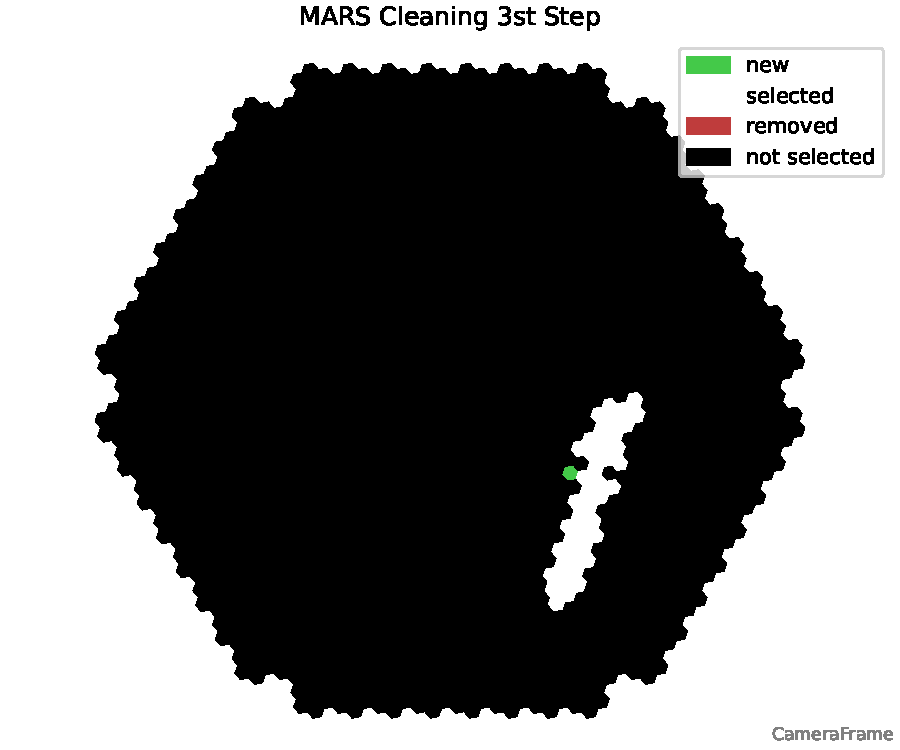
\includegraphics[width=\textwidth]{plots/cleaner_steps/mars_3.pdf}
    \end{subfigure}
    \caption{Visualization of the \mars{} algorithm for a \gls{mst} NectarCam image.}
    \label{fig:mars_cleaning}
\end{figure}

The \fact{} algorithm is a time-based cleaning algorithm that first selects all pixels that are above
the \texttt{core\_threshold}. Then, all pixels that have less than \(N\) neighbors are removed. The
\texttt{min\_number\_neighbors} parameter is set to \(\num{2}\) by default. For the third step, all pixels neighboring
the remaining pixels that are above the \texttt{boundary\_threshold} are selected. After that, all
pixels that have less than \(N\) neighbors and that have arrived within a given timeframe are removed.
The \texttt{time\_limit} parameter is set to \(\SI{5}{\nano\second}\) by default. Again, all pixels
with less than \(N\) neighbors are removed. The last step once again removes pixels with less than
\(N\) neighbors, arriving within the given time limit. The visualization of the algorithm is shown in
\autoref{fig:fact_cleaning} for the default values of the algorithm.

\begin{figure}
    \centering
    \begin{subfigure}[t]{0.32\textwidth}
        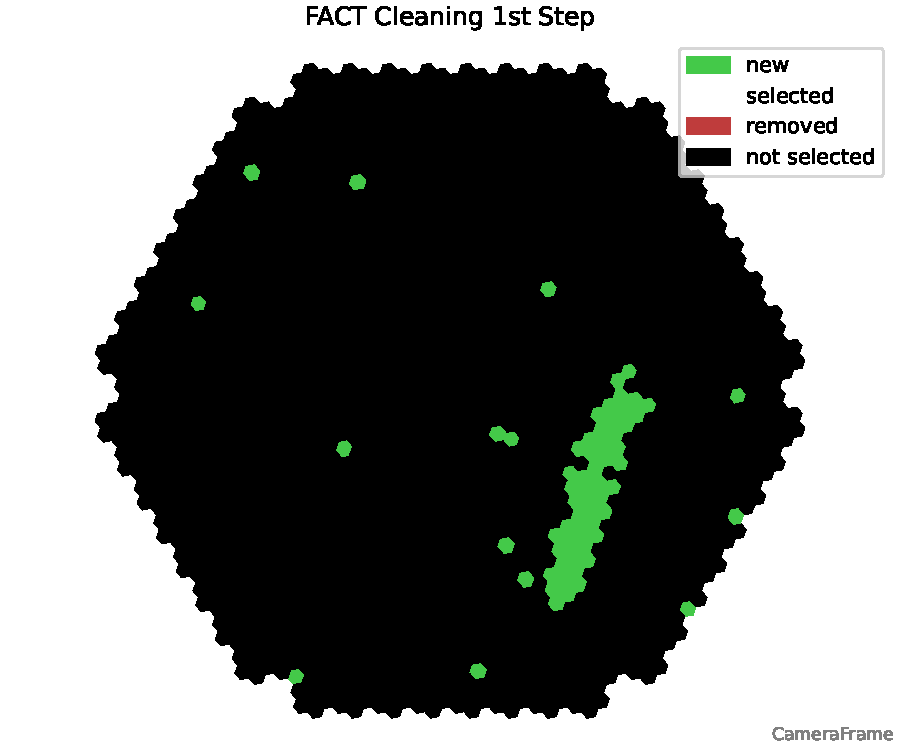
\includegraphics[width=\textwidth]{plots/cleaner_steps/fact_1.pdf}
    \end{subfigure}
    \hfill
    \begin{subfigure}[t]{0.32\textwidth}
        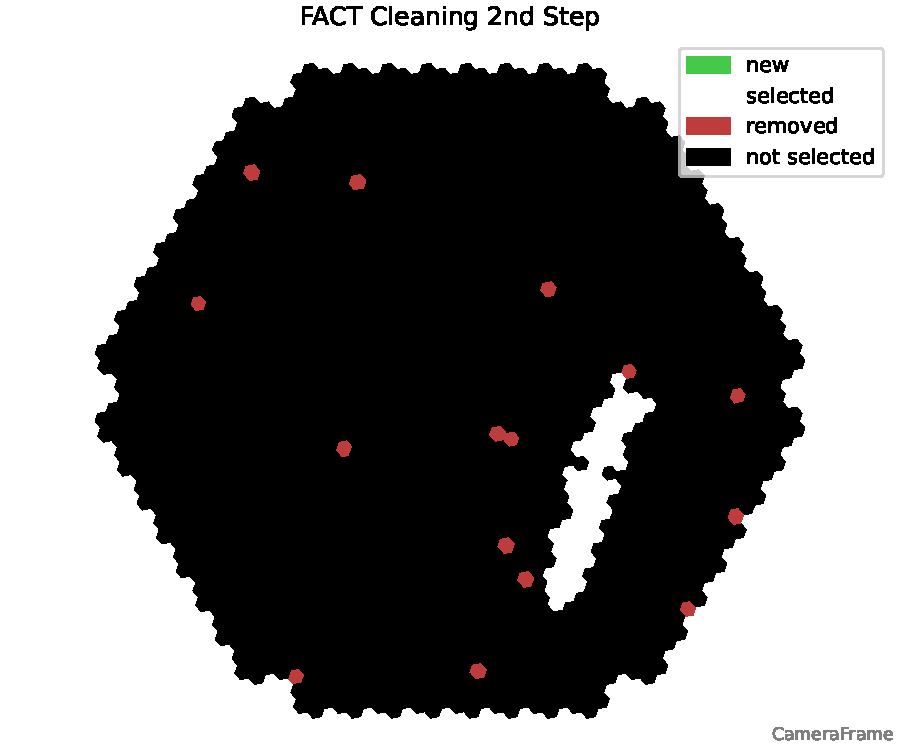
\includegraphics[width=\textwidth]{plots/cleaner_steps/fact_2.pdf}
    \end{subfigure}
    \hfill
    \begin{subfigure}[t]{0.32\textwidth}
        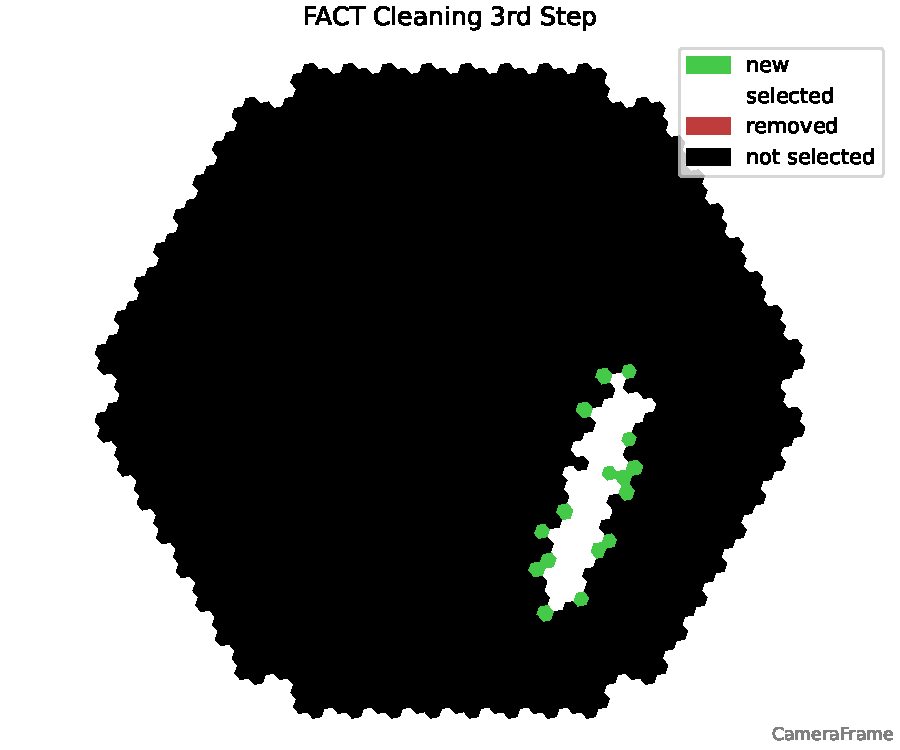
\includegraphics[width=\textwidth]{plots/cleaner_steps/fact_3.pdf}
    \end{subfigure}
    \begin{subfigure}[b]{0.32\textwidth}
        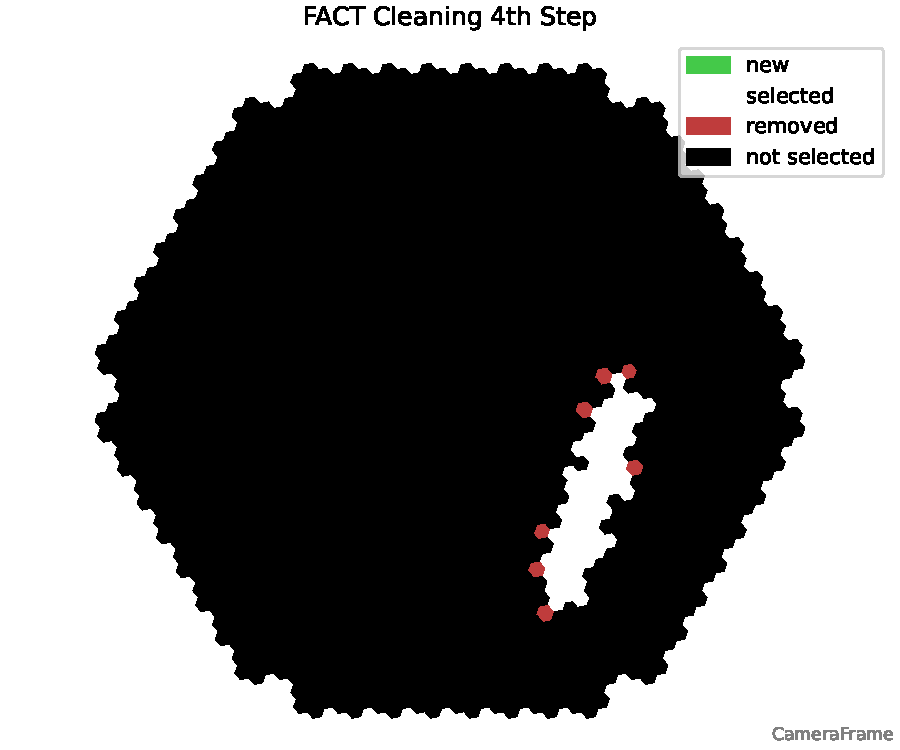
\includegraphics[width=\textwidth]{plots/cleaner_steps/fact_4.pdf}
    \end{subfigure}
    \hfill
    \begin{subfigure}[b]{0.32\textwidth}
        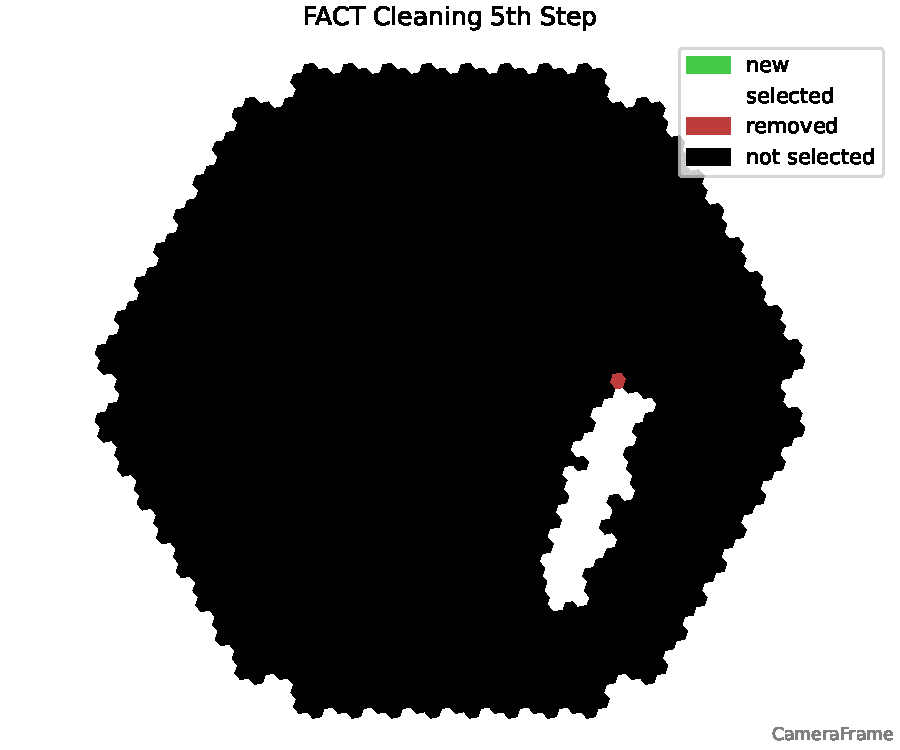
\includegraphics[width=\textwidth]{plots/cleaner_steps/fact_5.pdf}
    \end{subfigure}
    \hfill
    \begin{subfigure}[b]{0.32\textwidth}
        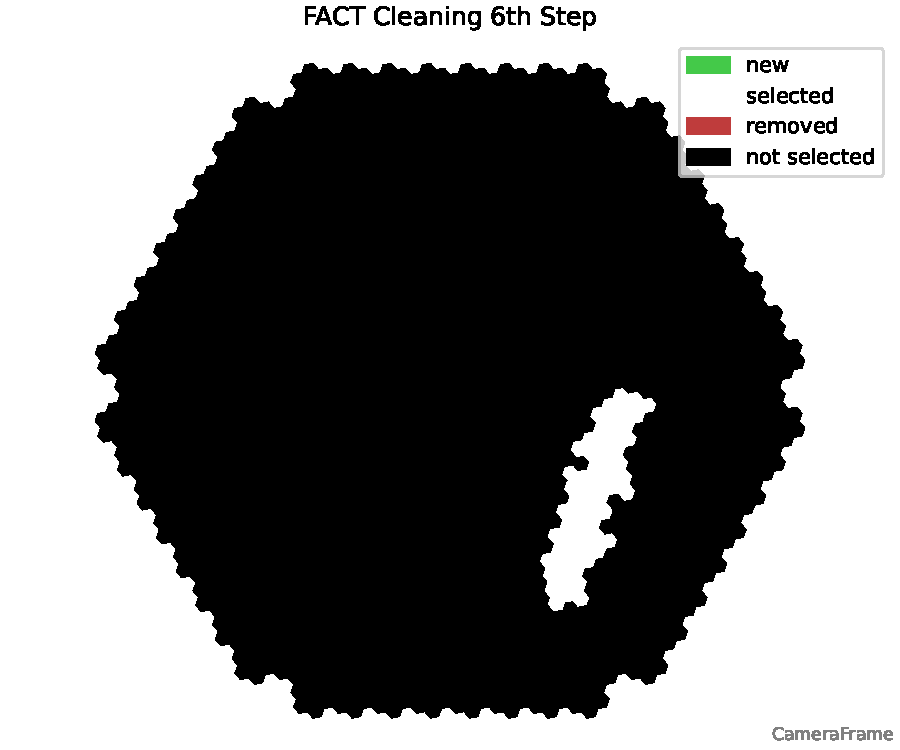
\includegraphics[width=\textwidth]{plots/cleaner_steps/fact_6.pdf}
    \end{subfigure}
    \caption{FACT cleaning steps}
    \label{fig:fact_cleaning}
\end{figure}

The \tcc{} algorithm is another time-based algorithm, coming from the \gls{magic} collaboration.
It first selects all pixels that are above the \texttt{core\_threshold}. Then, all pixels that have
less than \(N\) neighbors are removed. The \texttt{min\_number\_neighbors} parameter is set to \(\num{1}\) by default.
After that, all core pixels whose arrival times are within a given timeframe of the average arrival time.
This \texttt{time\_limit\_core} parameter is set to \(\SI{4.5}{\nano\second}\) by default. As a fourth step,
the \tcc{} algorithm finds all pixels above the \texttt{boundary\_threshold}. Then, all pixels with
less than \(N\) neighbors arriving within a given timeframe are removed. This \texttt{time\_limit\_boundary}
parameter is set to \(\SI{1.5}{\nano\second}\) by default. The visualization of the algorithm is shown in
\autoref{fig:tcc_cleaning} for the default values of the algorithm.

\begin{figure}
    \centering
    \begin{subfigure}[t]{0.32\textwidth}
        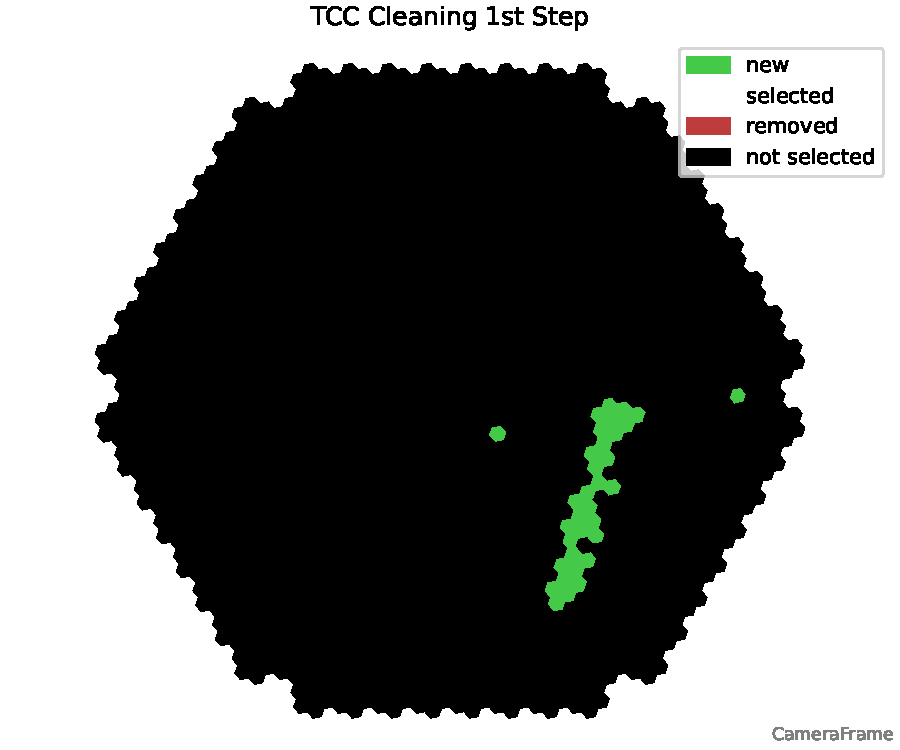
\includegraphics[width=\textwidth]{plots/cleaner_steps/tcc_1.pdf}
    \end{subfigure}
    \hfill
    \begin{subfigure}[t]{0.32\textwidth}
        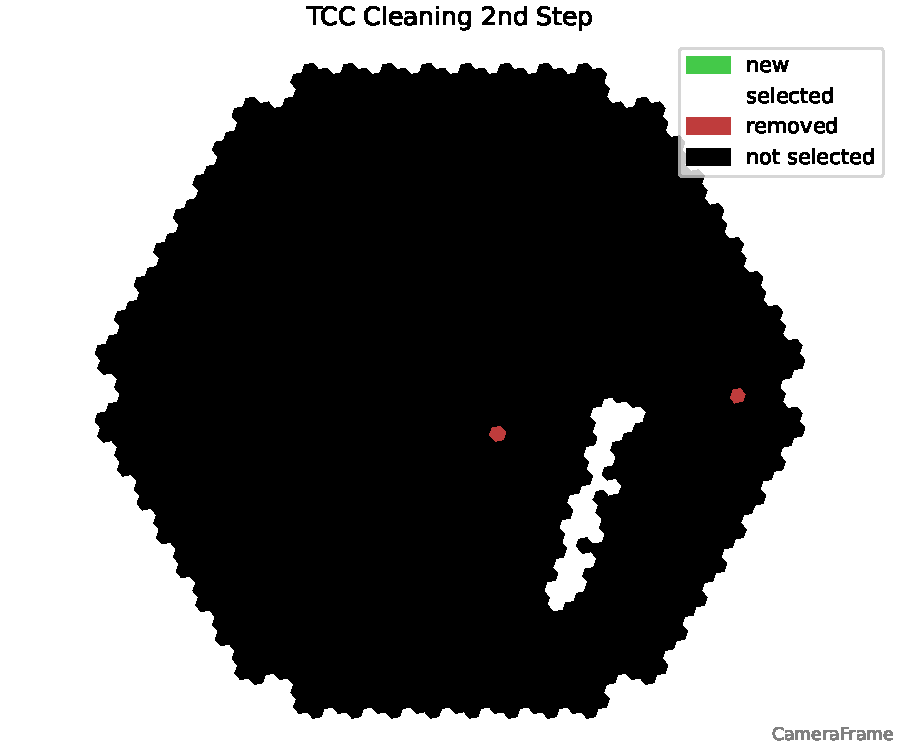
\includegraphics[width=\textwidth]{plots/cleaner_steps/tcc_2.pdf}
    \end{subfigure}
    \hfill
    \begin{subfigure}[t]{0.32\textwidth}
        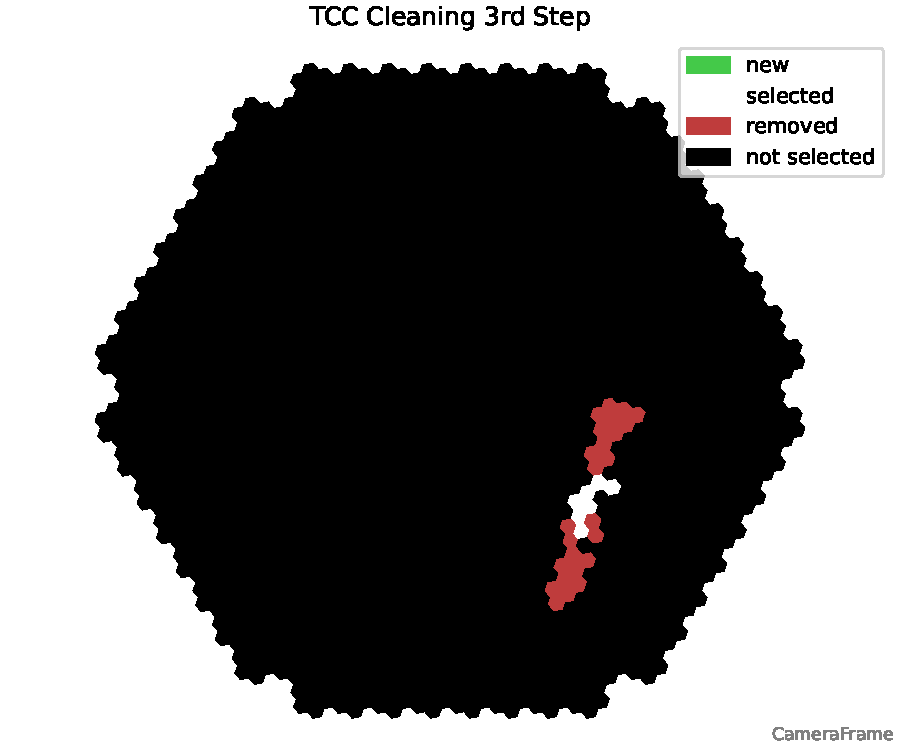
\includegraphics[width=\textwidth]{plots/cleaner_steps/tcc_3.pdf}
    \end{subfigure}
    \begin{subfigure}[]{0.32\textwidth}
        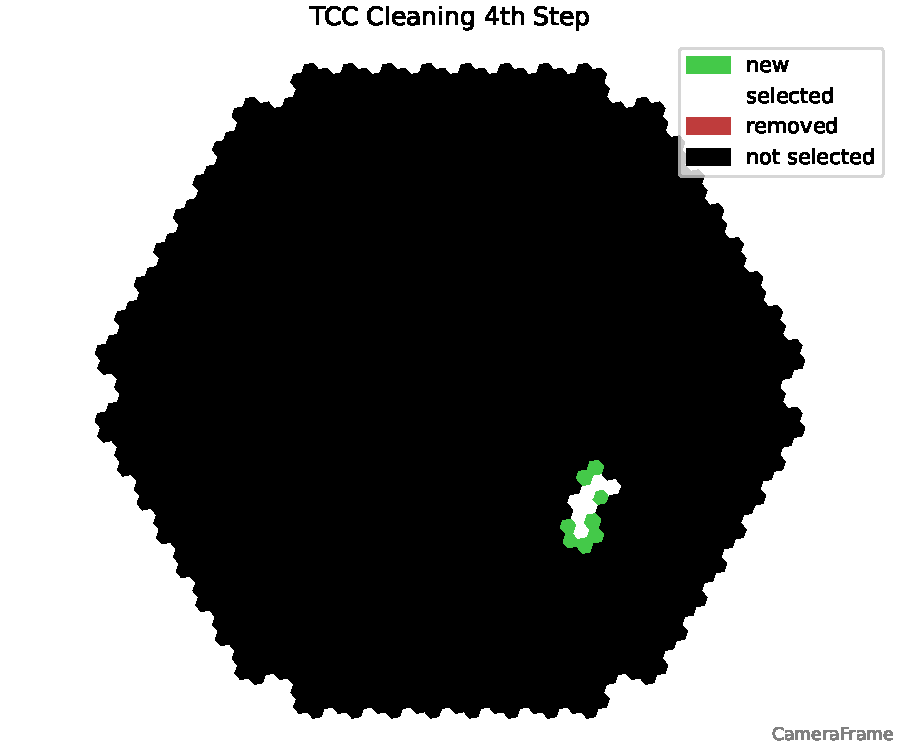
\includegraphics[width=\textwidth]{plots/cleaner_steps/tcc_4.pdf}
    \end{subfigure}
    \begin{subfigure}[]{0.32\textwidth}
        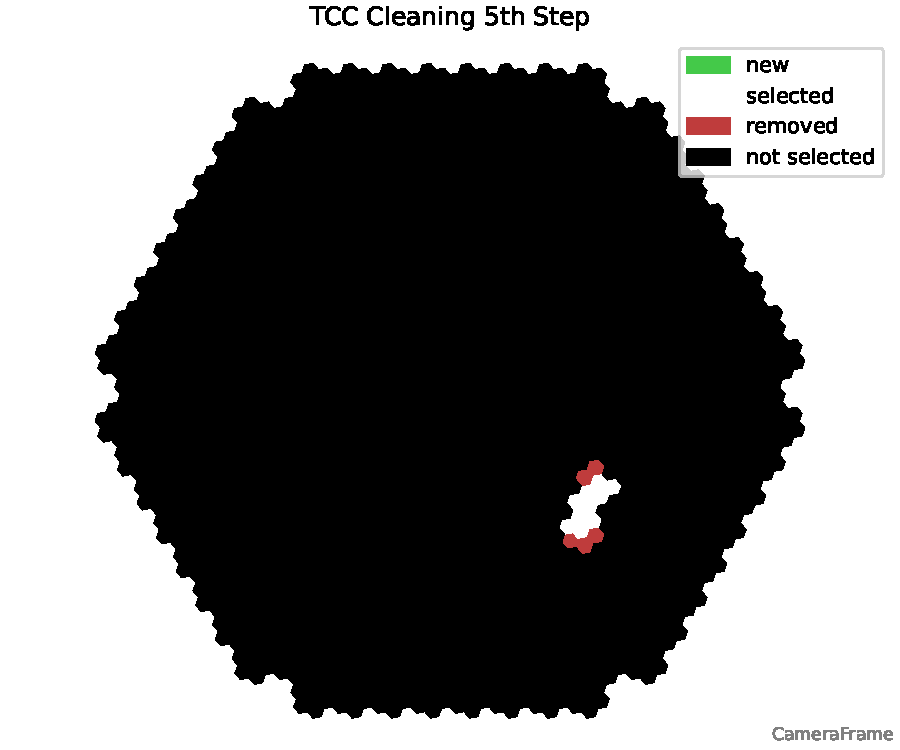
\includegraphics[width=\textwidth]{plots/cleaner_steps/tcc_5.pdf}
    \end{subfigure}
    \caption{TCC cleaning steps}
    \label{fig:tcc_cleaning}
\end{figure}

\section{Hyperparameters}
\label{sec:hyperparameters}

The hyperparameters of each cleaning algorithm are set in a specific \texttt{config} file. There,
the user can set and change the parameters, shown in \autoref{tab:hyperparameters}. \tailcuts{}
and \mars{} can be set-up with only three parameters: the \texttt{picture\_threshold}, the
\texttt{boundary\_threshold} and \texttt{min\_number\_picture\_neighbors}. The time-based algorithms
have additional parameters: a \texttt{time\_limit} for \fact{} and a \texttt{time\_limit\_core} as
well as a \texttt{time\_limit\_boundary} for \todo{watch out for text boundaries}\tcc{}.
\begin{table}
    \centering
    \caption{The four cleaning algorithms and their hyperparameters. Being the most basic algorithms,
    \tailcuts{} and \mars{} have only three parameters, while the \fact{} and \tcc{} algorithms have
    one and two additional time-based parameters, respectively. This table shows the default values,
    as they are implemented in the \ctapipe{} source code for version \texttt{0.15.1}.}
    \label{tab:hyperparameters}
    \begin{tabular}{l l l}
        \toprule
        \textbf{Cleaning Algorithm} & \textbf{Hyperparameter} & \textbf{Default Values} \\
        \midrule
        \tailcuts{} & \texttt{picture\_threshold}               & \qquad\(\SI{7}{\pe}\) \\
                    & \texttt{boundary\_threshold}              & \qquad\(\SI{5}{\pe}\) \\
                    & \texttt{min\_number\_picture\_neighbors}  & \qquad\(\num{0}\) \\
        \addlinespace[0.5em]
        \mars{}     & \texttt{picture\_threshold}               & \qquad\(\SI{7}{\pe}\) \\
                    & \texttt{boundary\_threshold}              & \qquad\(\SI{5}{\pe}\) \\
                    & \texttt{min\_number\_picture\_neighbors}  & \qquad\(\num{0}\) \\
        \addlinespace[0.5em]
        \fact{}     & \texttt{picture\_threshold}               & \qquad\(\SI{4}{\pe}\) \\
                    & \texttt{boundary\_threshold}              & \qquad\(\SI{2}{\pe}\) \\
                    & \texttt{time\_limit}                      & \qquad\(\SI{5}{\nano\second}\) \\
                    & \texttt{min\_number\_picture\_neighbors}  & \qquad\(\num{2}\) \\
        \addlinespace[0.5em]
        \tcc{}      & \texttt{picture\_threshold}               & \qquad\(\SI{7}{\pe}\) \\
                    & \texttt{boundary\_threshold}              & \qquad\(\SI{5}{\pe}\) \\
                    & \texttt{time\_limit\_core}                & \qquad\(\SI{4.5}{\nano\second}\) \\
                    & \texttt{time\_limit\_boundary}            & \qquad\(\SI{1.5}{\nano\second}\) \\
                    & \texttt{min\_number\_picture\_neighbors}  & \qquad\(\num{1}\) \\
        \bottomrule
  \end{tabular}
\end{table}

To find the optimal hyperparameters I used the \texttt{ParameterGrid} class from the
\todo{citation for sklearn?}\texttt{sklearn.model\_selection} module. The \texttt{ParameterGrid} class is useful to create a
dictionary of all possible combinations of a list of given parameters. These combinations are then
written to a config file and processed with \ctapipe{}. The output is hundreds of datasets equal to
the number of combinations of the given parameters, each with a different setting for the cleaning
performed on the data. Since it's impossible to find the optimal settings just by looking at the
cleaned images of the datasets, a combined metric is necessary to evaluate each cleaner's performance
for the parameter combinations.

In this work, I chose to first look at the efficiency \(n_{\mathrm{reco}} / n_{\mathrm{total}}\), where
\(n_{\mathrm{reco}}\) is the number of reconstructed events and \(n_{\mathrm{total}}\)
the total number of events in the dataset. By taking the mean of the efficiency, one can sort the
datasets by setting upper and lower bounds for the efficiency. For each interval, the mean angular
resolution is calculated. The dataset with the lowest mean angular resolution is the best performing
for each interval.

The intervals were chosen as \(\num{0.05}\), \ie \(\SI{5}{\percent}\), intervals, resulting in a total
of \(\num{20}\) intervals.

\chapter{Results}
\label{ch:results}

In this chapter, the results of the analysis are presented. First, I present the results of the
efficiency analysis in \autoref{sec:efficiency_angres}. The initial tests of parameter combinations
are based on a small dataset consisting of \(\num{20}\) runs, \ie \(\num{12668}\) events. This is
due to the number of parameter combinations that are tested, as more runs would increase the
processing time immensely. Furthermore, I show the results of the angular resolution for a combined
metric with the efficiency. Then, in \autoref{sec:metrics}, the metrics of each resulting combination
of hyperparameters are plotted. In \autoref{sec:performance}, the performance of each cleaning
algorithm compared to the default settings is shown. Finally, a comparison of the different
cleaning algorithms is provided in \autoref{sec:comparison}.


\section{Analysis of the Efficiency and the Angular Resolution}
\label{sec:efficiency_angres}

To narrow down possible candidates for the optimal hyperparameters, I first analyzed the efficiency
of the different cleaning algorithms. The efficiency is determined by the number of events that are
reconstructed after cleaning. For this work I chose \(\num{20}\) intervals within \(\num{0}\) and
\(\num{1}\) with a step size of \(\num{0.05}\). The number of reconstructed events \(n_{\mathrm{reco}}\)
and the total number of events \(n_{\mathrm{total}}\) are binned per energy and the efficiency is then
calculated as
\begin{equation}\label{eq:efficiency_sum}
    \eff = \frac{\sum_{N} n_{\mathrm{reco}}}{\sum_{\mathrm{N}} n_{\mathrm{total}}},
\end{equation}
with \(N\) being the number of bins. For each interval only those datasets are selected, where the efficiency
lies between the lower and upper bound of the interval. Then the minimum angular resolution is
determined for each interval. The parameters of these datasets are then selected to be the optimal
parameters for each cleaning algorithm. This not only allows for a comparison of the cleaners but also
a decision on a trade-off between the efficiency and the angular resolution, namely having a better
angular resolution, but a lower efficiency or a higher efficiency but a higher and therefore worse
angular resolution. The results for the efficiency are listed in \autoref{tab:efficiency} and
the results for the mean angular resolution in \autoref{tab:angres}.

As one can see, not all cleaning algorithms have valid values for each interval, peaking at a maximum
of around \(\SIrange{40}{45}{\percent}\) of successfully reconstructed events. This is because not
all events are stereo events, \ie events, where two or more telescopes were triggered, which is a
requirement for the reconstruction.
The remaining events are therefore mono events and do not contribute to either the efficiency or the
angular resolution. The efficiency would be higher, of course, for a full-array analysis, but that would
mean also including \glspl{lst} data\footnote{which was left out due to time limitations, see \autoref{ch:conclusions}.},
which for this work would not help find the optimal parameters, since it is better to analyze the telescope
types separately. The reason for the latter is, that optimizing the telescopes by type would lead to
better results for the hyperparameters.
\begin{table}
    \centering
    \caption{The results of the analysis for the efficiency of each cleaning algorithm taken over all
    energy bins. The table lists the lower and upper limits of each efficiency
    interval. The efficiency is calculated according to \autoref{eq:efficiency_sum} and
    each listed efficiency is the one where the mean angular resolution is minimal for the given
    interval. Notice how not all cleaning algorithms have valid results for all efficiency intervals, due to not all
    events being stereo events.}
    \label{tab:efficiency}
    \rowcolors{0}{white!92!black}{}
    \begin{tabular}{S[table-format=1.2] S[table-format=1.2] S[table-format=1.3] S[table-format=1.3] S[table-format=1.3] S[table-format=1.3]}
        \hiderowcolors
        & & \multicolumn{4}{c}{Mean Efficiency} \\
        {$\eff_{\mathrm{lower}}$} & {$\eff_{\mathrm{upper}}$} & {Tailcuts} & {MARS} & {FACT} & {TCC} \\
        \addlinespace[0.5em]
        \showrowcolors
        % \input{build/efficiency.txt}
        0.00 & 0.05 &       &       & 0.007 &       \\
        0.05 & 0.10 &       &       & 0.051 & 0.070 \\
        0.10 & 0.15 & 0.121 & 0.122 & 0.141 & 0.121 \\
        0.15 & 0.20 & 0.177 & 0.179 & 0.178 & 0.176 \\
        0.20 & 0.25 & 0.242 & 0.244 & 0.250 & 0.248 \\
        0.25 & 0.30 & 0.296 & 0.297 & 0.254 & 0.263 \\
        0.30 & 0.35 & 0.307 & 0.306 & 0.340 & 0.311 \\
        0.35 & 0.40 & 0.365 & 0.380 & 0.388 & 0.375 \\
        0.40 & 0.45 & 0.401 & 0.410 & 0.405 & 0.401 \\
    \end{tabular}
\end{table}

\begin{table}
    \centering
    \caption{The results of the analysis for the mean angular resolution of each cleaning algorithm.
    The table lists the lower and upper limits of each efficiency interval. The angular resolution listed
    is the minimum mean angular resolution of the respective efficiency interval. The corresponding efficiency
    values are listed in \autoref{tab:efficiency}. Notice how not all cleaning algorithms have valid results for all efficiency intervals, due to not all
    events being stereo events.}
    \label{tab:angres}
    \rowcolors{0}{white!92!black}{}
    \begin{tabular}{S[table-format=1.2] S[table-format=1.2] S[table-format=1.3] S[table-format=1.3] S[table-format=1.3] S[table-format=1.3]}
        \hiderowcolors
        & & \multicolumn{4}{c}{Mean Angular Resolution\(\;/\; \si{\degree}\)} \\
        {$\eff_{\mathrm{lower}}$} & {$\eff_{\mathrm{upper}}$} & {Tailcuts} & {MARS} & {FACT} & {TCC} \\
        \addlinespace[0.5em]
        \showrowcolors
        % \input{build/angular_resolution.tex}
        0.00 & 0.05 &       &       & 0.244 &       \\
        0.05 & 0.10 &       &       & 0.428 & 0.413 \\
        0.10 & 0.15 & 0.358 & 0.291 & 0.415 & 0.396 \\
        0.15 & 0.20 & 0.308 & 0.282 & 0.367 & 0.340 \\
        0.20 & 0.25 & 0.334 & 0.332 & 0.403 & 0.388 \\
        0.25 & 0.30 & 0.346 & 0.356 & 0.366 & 0.386 \\
        0.30 & 0.35 & 0.357 & 0.343 & 0.365 & 0.383 \\
        0.35 & 0.40 & 0.395 & 0.395 & 0.404 & 0.390 \\
        0.40 & 0.45 & 0.432 & 0.424 & 0.420 & 0.427 \\
    \end{tabular}
\end{table}
The results listed in the tables show that there is a clear trade-off in choosing between efficiency and angular resolution.
As such, for further comparison of the cleaning algorithms, the corresponding datasets for the efficiency and
the angular resolution are plotted in \autoref{fig:efficiency_angres} for the intervals
\([\num{0.25}, \num{0.30}]\) and \([\num{0.45}, \num{0.50}]\). The reason for this is that these are
the minimum and maximum intervals \wrt the efficiency, where all cleaners have valid values.
Furthermore, the mean angular resolution is plotted against the efficiency in \autoref{fig:ar_vs_eff}.
\vspace{-0.2cm}
\begin{figure}
    \centering
    \begin{subfigure}{0.48\textwidth}
        \centering
        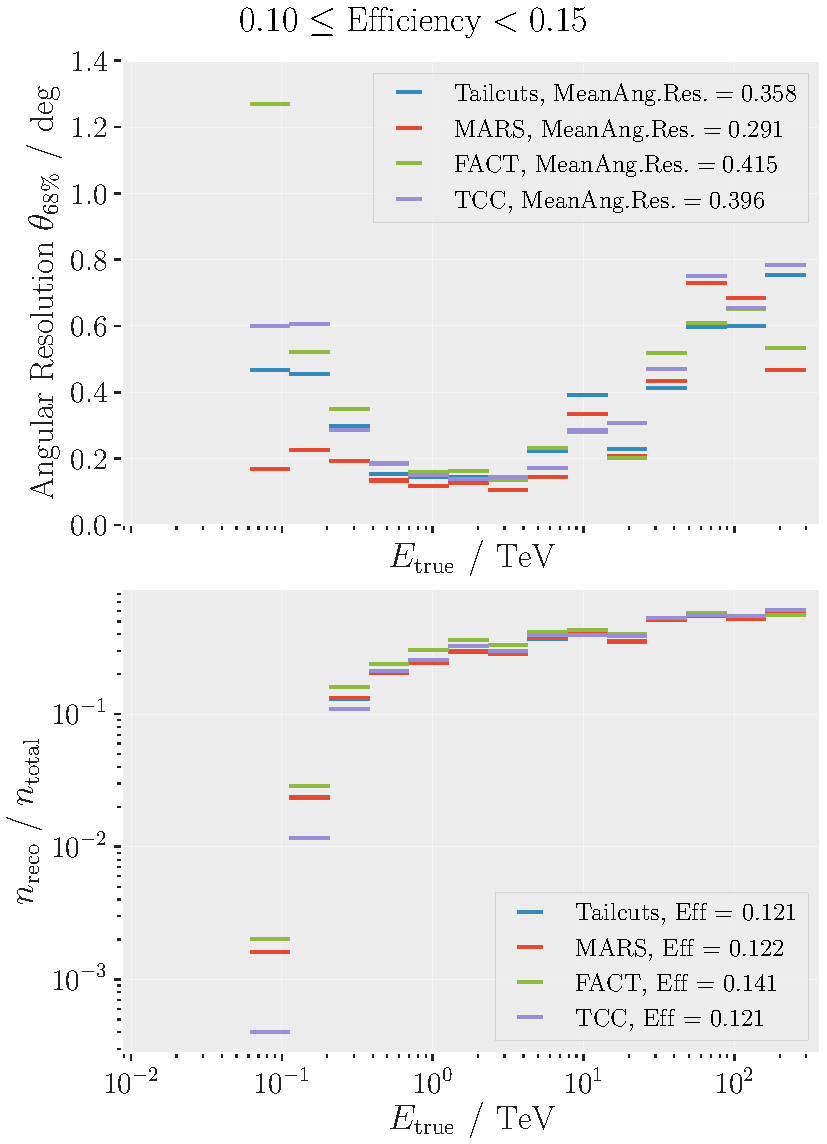
\includegraphics[width=0.85\textwidth]{plots/ar_aeff/AR_Aeff_MST_0.10_0.15.pdf}
    \end{subfigure}
    \hfill
    \begin{subfigure}{0.48\textwidth}
        \centering
        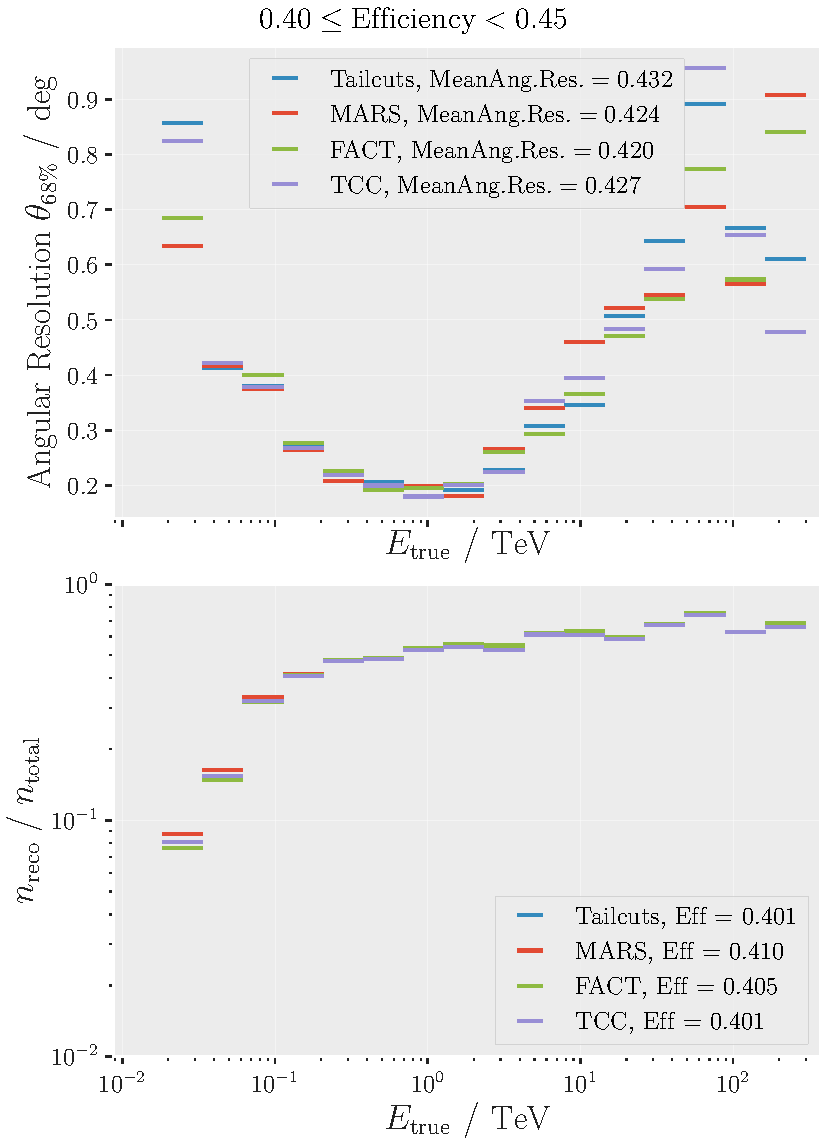
\includegraphics[width=0.85\textwidth]{plots/ar_aeff/AR_Aeff_MST_0.40_0.45.pdf}
    \end{subfigure}
    \caption{Mean angular resolution and efficiency for the MST simulation binned per energy. Notice
    the decrease in the scattering of the mean angular resolution at medium to
    medium-high energies at higher efficiencies in the plots on the right.\vspace{-0.5cm}}
    \label{fig:efficiency_angres}
\end{figure}
\begin{figure}[!htbp]
    \centering
    \includegraphics[width=0.75\textwidth]{build/ar_vs_eff.pdf}
    \caption{Angular resolution plotted against the efficiency between \(\num{0.355}\) and \(\num{0.485}\).}
    \label{fig:ar_vs_eff}
\end{figure}


\section{Metrics of the Cleaning Algorithms}
\label{sec:metrics}
\glsreset{tp}\glsreset{fp}\glsreset{fn}\glsreset{tn}
Concerning the metrics, I first analyzed the parameter combinations of all settings found in \autoref{sec:efficiency_angres}. First,
the number of the \gls{tp}, \gls{fp}, \gls{fn} and \gls{tn} values is calculated per event. Then,
those values are summed up for each cleaning algorithm and the metrics are calculated as shown in
\autoref{tab:metrics}.

The metrics for each parameter combination are first compared for each cleaning algorithm respectively,
to determine the best setting within a set of parameter combinations. The results are then plotted in
\Autoref{fig:metrics_tail, fig:metrics_mars, fig:metrics_fact, fig:metrics_tcc}
and are shown with specific IDs they were given when the datasets were processed with \ctapipe.
This improves readability as opposed to writing out the full settings. The hyperparameters for the best performing
IDs of all algorithms are listed in \autoref{tab:best_parameters}.

While all settings perform well w.\,r.\,t., for example, the \gls{tnr}, one can see from the results, that for all cleaning
algorithms, the best parameter combination is the one where the \gls{tpr}, the \gls{acc} and the \gls{ba}
are the highest. These settings are the ones that correspond to the highest efficiency.
The values for each respective metric and cleaning algorithm are listed in
\Autoref{tab:metrics_tail, tab:metrics_mars, tab:metrics_fact, tab:metrics_tcc} respectively, while
a comparison of the cleaners against each other is shown in \autoref{sec:comparison}.
\begin{table}
    \centering
    \caption{Results for the metrics of \tailcuts{}. One can see, that the best results are obtained
    for the setting with ID~101.}
    \label{tab:metrics_tail}
    \rowcolors{0}{white!92!black}{}
    \adjustbox{varwidth=\linewidth,scale=0.9}{%
    \begin{tabular}{r S[table-format=1.4] S[table-format=1.4] S[table-format=1.4] S[table-format=1.4] S[table-format=1.4] S[table-format=1.4] S[table-format=1.4]}
        \hiderowcolors
        {ID} & \acrshort{tpr} & \acrshort{tnr} & \acrshort{fnr} & \acrshort{acc} & \acrshort{ba} \\
        \addlinespace[0.5em]
        \showrowcolors
        % \input{build/metrics_tail.txt} %% kinda broken atm
        118 & 0.0972 & 1.0000 & 0.9028 & 0.9256 & 0.5486 \\
         51 & 0.1231 & 1.0000 & 0.8769 & 0.9256 & 0.5615 \\
        140 & 0.1460 & 1.0000 & 0.8540 & 0.9256 & 0.5730 \\
        141 & 0.1660 & 1.0000 & 0.8340 & 0.9283 & 0.5830 \\
         81 & 0.1854 & 1.0000 & 0.8146 & 0.9288 & 0.5927 \\
         47 & 0.2268 & 1.0000 & 0.7732 & 0.9332 & 0.6134 \\
        101 & 0.3169 & 0.9997 & 0.6831 & 0.9418 & 0.6583 \\
    \end{tabular}}
\end{table}

\begin{figure}
    \centering
    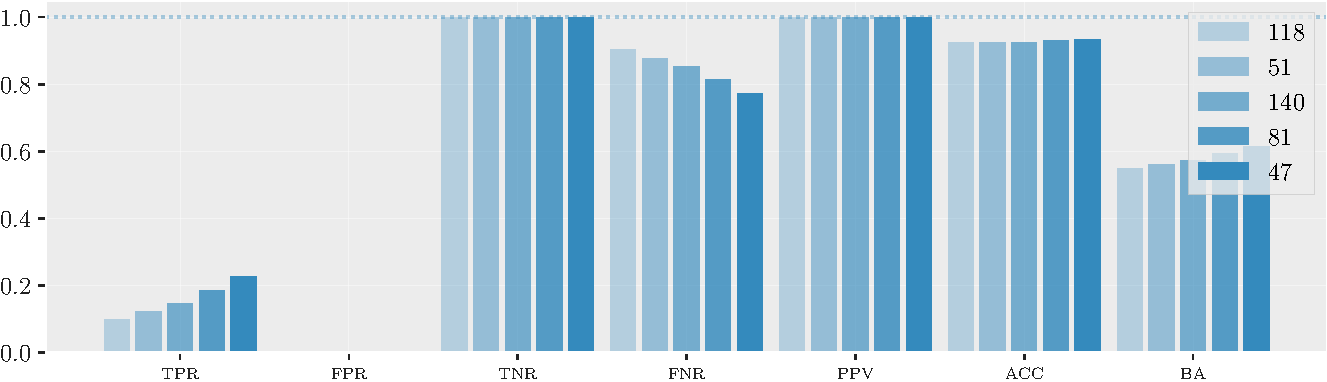
\includegraphics[width=0.95\textwidth]{build/metrics_tailcuts.pdf}
    \caption{Metrics for \tailcuts{}. It can be seen, that the cleaning setting with ID 47 performs
    best in terms of the true positive rate, accuracy and balanced accuracy, making it the best
    setting of the five parameter combinations.}
    \label{fig:metrics_tail}
\end{figure}

\begin{table}
    \centering
    \caption{Results for the metrics of \mars{}. The last row (ID~10) shows a significant increase in the \gls{tpr}
    and therefore decrease in \gls{fnr} and another significant increase in the \gls{ba} value. Since
    this specific parameter combination also corresponds to a mean angular resolution an order higher
    than the rest, I chose to select the second highest performing setting (ID~15) for further analysis
    instead.}
    \label{tab:metrics_mars}
    \rowcolors{0}{white!92!black}{}
    \begin{tabular}{r S[table-format=1.4] S[table-format=1.4] S[table-format=1.4] S[table-format=1.4] S[table-format=1.4] S[table-format=1.4] S[table-format=1.4]}
        \hiderowcolors
        ID & \acrshort{tpr} & \acrshort{tnr} & \acrshort{fnr} & \acrshort{acc} & \acrshort{ba} \\
        \addlinespace[0.5em]
        \showrowcolors
        \input{build/metrics_mars.txt}\\
    \end{tabular}
\end{table}

\begin{figure}
    \centering
    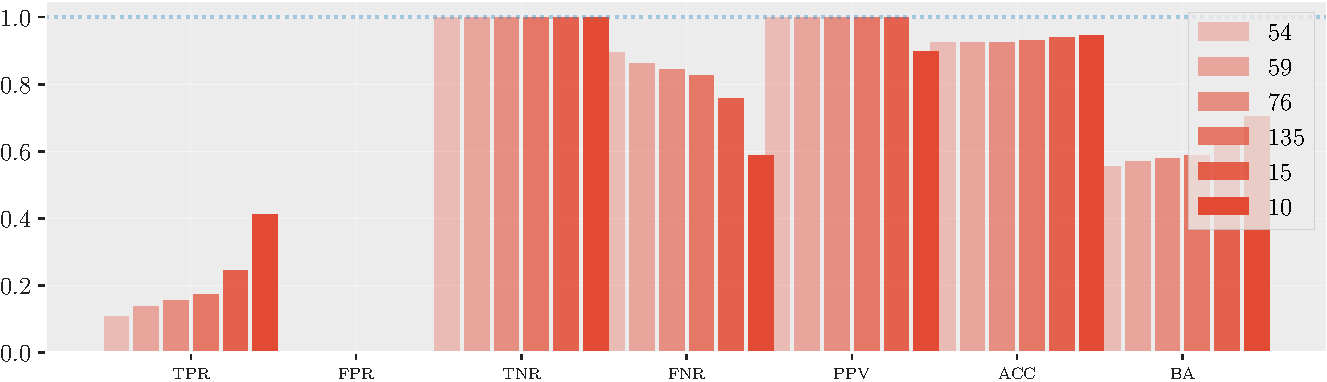
\includegraphics[width=\textwidth]{build/metrics_mars.pdf}
    \caption{Metrics for \mars{}. The results show, that the cleaning setting with ID~13 performs
    best in terms of the true positive rate, accuracy and balanced accuracy, making it the best
    setting of the five parameter combinations \wrt the metrics.}
    \label{fig:metrics_mars}
\end{figure}

\begin{table}
    \centering
    \caption{Results for the metrics of \fact{}. One can see, that the best results are obtained
    for the settings with ID~974.}
    \label{tab:metrics_fact}
    \rowcolors{0}{white!92!black}{}
    \begin{tabular}{r S[table-format=1.4] S[table-format=1.4] S[table-format=1.4] S[table-format=1.4] S[table-format=1.4] S[table-format=1.4] S[table-format=1.4]}
        \hiderowcolors
        ID & \acrshort{tpr} & \acrshort{tnr} & \acrshort{fnr} & \acrshort{acc} & \acrshort{ba} \\
        \addlinespace[0.5em]
        \showrowcolors
        \input{build/metrics_fact.txt}
    \end{tabular}
\end{table}

\begin{figure}
    \centering
    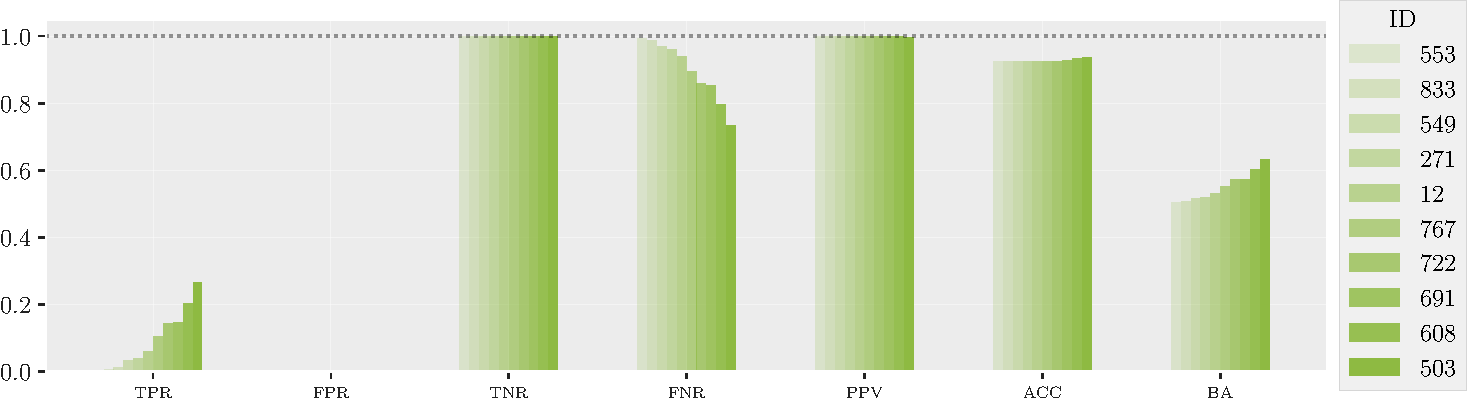
\includegraphics[width=\textwidth]{build/metrics_fact.pdf}
    \caption{Metrics for \fact{}. The cleaning setting with ID~947 performs
    best in terms of the number of true positives, accuracy and balanced accuracy, making it the best
    setting of the nine parameter combinations.}
    \label{fig:metrics_fact}
\end{figure}

\begin{table}
    \centering
    \caption{Results for the metrics of \tcc{}. The best results are obtained
    for the setting with ID~1954.}
    \label{tab:metrics_tcc}
    \rowcolors{0}{white!92!black}{}
    \begin{tabular}{r S[table-format=1.4] S[table-format=1.4] S[table-format=1.4] S[table-format=1.4] S[table-format=1.4] S[table-format=1.4] S[table-format=1.4] }
        \hiderowcolors
        ID & \acrshort{tpr} & \acrshort{tnr} & \acrshort{fnr} & \acrshort{acc} & \acrshort{ba} \\
        \addlinespace[0.5em]
        \showrowcolors
        \input{build/metrics_tcc.txt}
    \end{tabular}
\end{table}

\begin{figure}
    \centering
    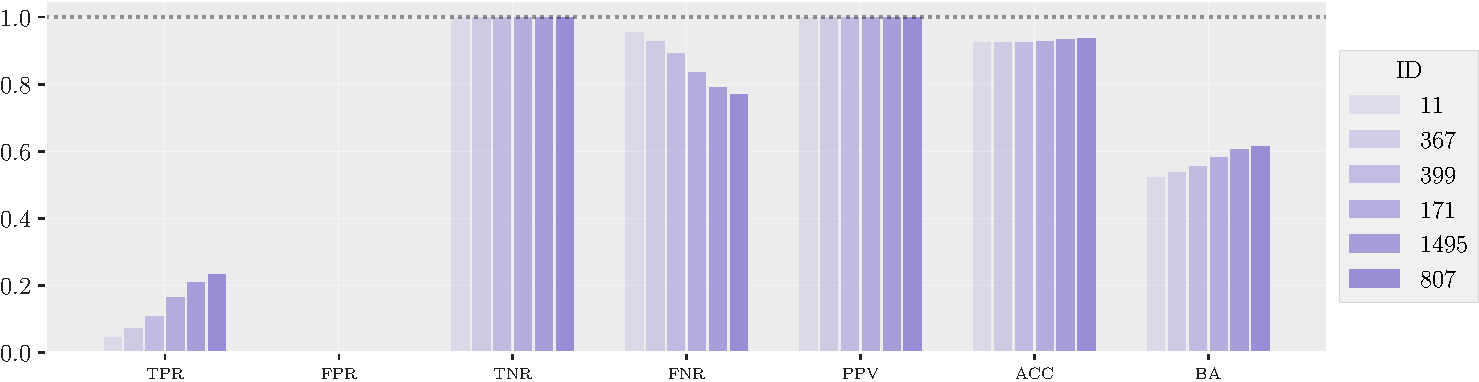
\includegraphics[width=\textwidth]{build/metrics_tcc.pdf}
    \caption{Metrics for the \tcc{}. The cleaning setting with ID~1954 performs
    best in terms of the number of true positives, accuracy and balanced accuracy, making it the best
    setting of the eight parameter combinations.}
    \label{fig:metrics_tcc}
\end{figure}

\begin{table}
    \centering
    \caption{Best performing IDs and the corresponding hyperparameters for each respective cleaner.
    Note, that, as discussed above, the best performing ID \wrt
    the metrics for \mars{} is, in fact, not the best, but the second best. This is because the mean angular resolution is
    an order of magnitude better for ID~15 than the one for ID~10. For better readability, the names
    of the algorithms are shortened. Listed are the core threshold \(Q_c\), the boundary threshold \(Q_b\),
    the minimum number of neighbors and where applicable the time limit \(t\) and core and boundary time limits
    \(t_c\) and \(t_b\).}
    \label{tab:best_parameters}
    \rowcolors{0}{white!92!black}{}
    \begin{tabular}{c S[table-format=2.0] S[table-format=1.3]
        S[table-format=1.3] S[table-format=1.0] S[table-format=2.1] S[table-format=2.1] S[table-format=2.1]}
        \hiderowcolors
        {Cleaning Algorithm} & {ID} & {\(Q_c \;/\; \si{\pe}\)} & {\(Q_b \;/\; \si{\pe}\)} & {Min. Neigh.} &
        {\(t \;/\; \si{\nano\second}\)} & {\(t_c \;/\; \si{\nano\second}\)} & {\(t_b \;/\; \si{\nano\second}\)} \\
        \addlinespace[0.5em]
        \showrowcolors
        Tailcuts &  47 & 6.200 & 4.650 & 2 &      &      &      \\
        MARS     &  15 & 6.700 & 4.467 & 1 &      &      &      \\
        FACT     & 503 & 6.700 & 3.350 & 1 & 12.0 &      &      \\
        TCC      & 807 & 6.700 & 4.467 & 1 &      & 15.0 & 12.0 \\
    \end{tabular}
\end{table}

\section{Performance Compared to the Default Settings}
\label{sec:performance}

Now, with a setting selected for each cleaner, it is reasonable to compare
the performance to the default settings, that are implemented in the \ctapipe{} source code
(see \autoref{tab:hyperparameters}). First, the relative angular resolution
\begin{equation}
    \theta_\text{rel} = \frac{\theta_{\SI{68}{\percent}}}{\theta_{\SI{68}{\percent},\,\text{base}}}
\end{equation}
is computed for the default (base) settings and the selected settings for each cleaner.
The results are shown in \autoref{fig:rel_angres} for the same efficiency intervals
as in \autoref{fig:efficiency_angres}. One can see, that especially for the interval
\([0.45, 0.5)\) and at medium to high energies, \tcc{} performs fairly well compared to the default settings.
The other algorithms perform only slightly better than the default settings at a performance gain
of about \(\SI{10}{\percent}\).

Furthermore, the metrics of the hyperparameters determined in this work can be compared to the
metrics of the default settings. The results are shown in \autoref{fig:metrics_comparison} with the
values of the metrics being listed in \autoref{tab:metrics_default}. The values for the selected
settings in this work are listed in \autoref{tab:metrics_all}.
\fact{} performs worse than its default setting \wrt the metrics, especially in terms of
\gls{tpr} and \gls{ba}. This might be due to the higher core and boundary thresholds compared to the
default values, as lower values would allow selecting more pixels. \tcc{}, however, performs
significantly better than the default settings, especially in terms of \gls{tpr} and \gls{ba}, but
also slightly better in terms of the \gls{acc} metric.
\begin{figure}
    \centering
    \includegraphics[width=\textwidth]{build/metrics_baseline.pdf}
    \caption{Metrics for the default (baseline) settings compared to the settings determined in this work.
    One can see that an improvement was reached for \tcc, especially in terms of \gls{tpr} and \gls{ba}, while
    \fact{} performs worse than its default implementation.}
    \label{fig:metrics_comparison}
\end{figure}
\begin{figure}
    \centering
    \begin{subfigure}[t]{0.45\textwidth}
        \centering
        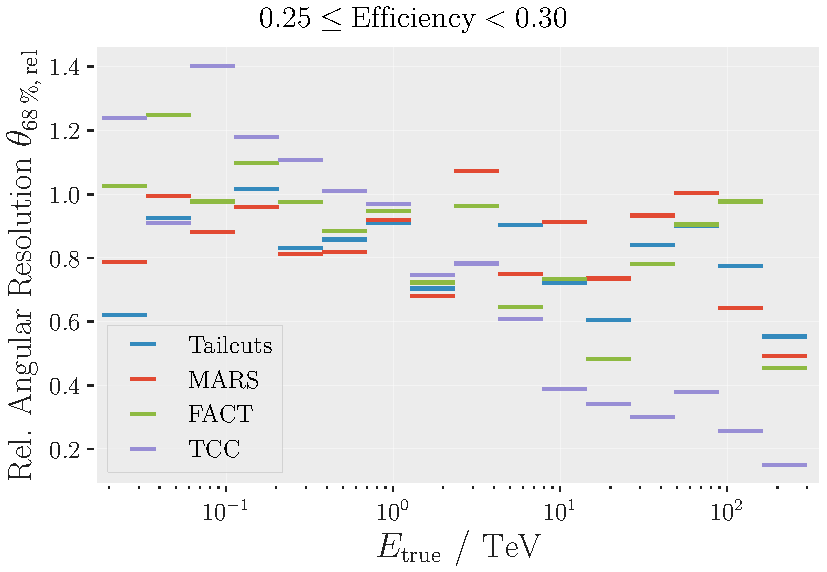
\includegraphics[width=\textwidth]{plots/ar_aeff/Rel_AR_0.25_0.30_base.pdf}
    \end{subfigure}
    \hfill
    \begin{subfigure}[t]{0.45\textwidth}
        \centering
        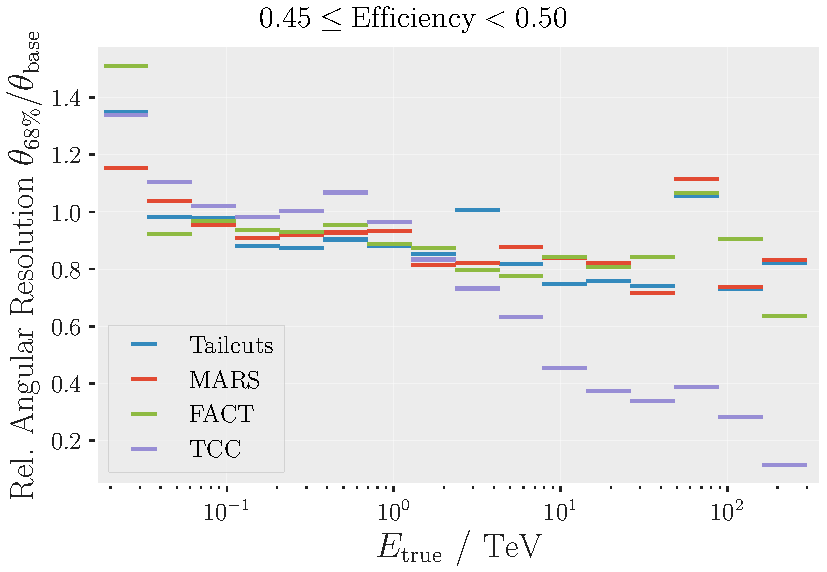
\includegraphics[width=\textwidth]{plots/ar_aeff/Rel_AR_0.45_0.50_base.pdf}
    \end{subfigure}
    \caption{Relative angular resolution for the default settings and the selected settings for each cleaner.
    \tcc{} outperforms the default values with the new settings, while the other algorithms improve only slightly.}
    \label{fig:rel_angres}
\end{figure}

\begin{table}
    \centering
    \caption{Metrics for the default (baseline) settings. The metrics show that \fact{}
    performs well even in its default settings and also better than with the hyperparameters
    determined in this work. \tcc{}, however, performs better with the hyperparameters listed in
    \autoref{tab:best_parameters} \wrt the metrics.}
    \label{tab:metrics_default}
    \rowcolors{0}{white!92!black}{}
    \begin{tabular}{c S[table-format=1.4] S[table-format=1.4] S[table-format=1.4]
        S[table-format=1.4] S[table-format=1.4] S[table-format=1.4] S[table-format=1.4]}
        \hiderowcolors
        {Cleaning Algorithm} & {\acrshort{tpr}} & {\acrshort{fpr}} & {\acrshort{tnr}} &
        {\acrshort{fnr}} & {\acrshort{ppv}} & {\acrshort{acc}} & {\acrshort{ba}} \\
        \addlinespace[0.5em]
        \showrowcolors
        Tailcuts & 0.2316 & 0.0000 & 1.0000 & 0.7684 & 0.9971 & 0.9358 & 0.6158 \\
        MARS     & 0.2346 & 0.0000 & 1.0000 & 0.7654 & 0.9970 & 0.9358 & 0.6173 \\
        FACT     & 0.3261 & 0.0002 & 0.9998 & 0.6739 & 0.9864 & 0.9429 & 0.6629 \\
        TCC      & 0.1790 & 0.0000 & 1.0000 & 0.8210 & 0.9995 & 0.9299 & 0.5895 \\

    \end{tabular}
\end{table}

\section{Comparison of the Cleaning Algorithms}
\label{sec:comparison}

As of writing this thesis, the cleaning algorithms discussed in this thesis are the only ones implemented
in the \ctapipe{} source code. With the determined hyperparameters, I decided to compare the performance of all
four cleaners. I once again decided to use the settings selected in \autoref{sec:metrics} for each algorithm
and look at the metrics. The metrics of all four algorithms are shown in \autoref{fig:metrics_all}.
The corresponding values are listed in \autoref{tab:metrics_all}.

One can see, that \fact{} performs best in terms of \gls{tpr} and \gls{ba}, while \mars{} and
\tailcuts{} perform well on \gls{acc} and \gls{ppv} respectively. Overall, however, \fact{} seems
to be a good choice for cleaning since it performs reasonably well even on \gls{acc} and \gls{ppv}.


\begin{table}
    \centering
    \caption{Metrics for the selected settings of each cleaning algorithm. Out of these
    four algorithms, \fact{} performs best in terms of \gls{tpr} and \gls{ba}, while \mars{} and
    \tailcuts{} perform well on \gls{acc} and \gls{ppv} respectively. \fact{}, however, performs
    reasonably well in the scope of the resulting metrics of this work and is, therefore, a good
    overall choice for cleaning.}
    \label{tab:metrics_all}
    \rowcolors{0}{white!92!black}{}
    \begin{tabular}{c S[table-format=1.4] S[table-format=1.4] S[table-format=1.4]
        S[table-format=1.4] S[table-format=1.4] S[table-format=1.4] S[table-format=1.4]}
        \hiderowcolors
        {Cleaning Algorithm} & {\acrshort{tpr}} & {\acrshort{fpr}} & {\acrshort{tnr}} &
        {\acrshort{fnr}} & {\acrshort{ppv}} & {\acrshort{acc}} & {\acrshort{ba}} \\
        \addlinespace[0.5em]
        \showrowcolors
        Tailcuts & 0.2268 & 0.0000 & 1.0000 & 0.7732 & 0.9994 & 0.9332 & 0.6134 \\
        MARS     & 0.2433 & 0.0000 & 1.0000 & 0.7567 & 0.9985 & 0.9380 & 0.6216 \\
        FACT     & 0.2655 & 0.0000 & 1.0000 & 0.7345 & 0.9968 & 0.9369 & 0.6327 \\
        TCC      & 0.2314 & 0.0000 & 1.0000 & 0.7686 & 0.9989 & 0.9364 & 0.6157 \\
    \end{tabular}
\end{table}

\begin{figure}
    \centering
    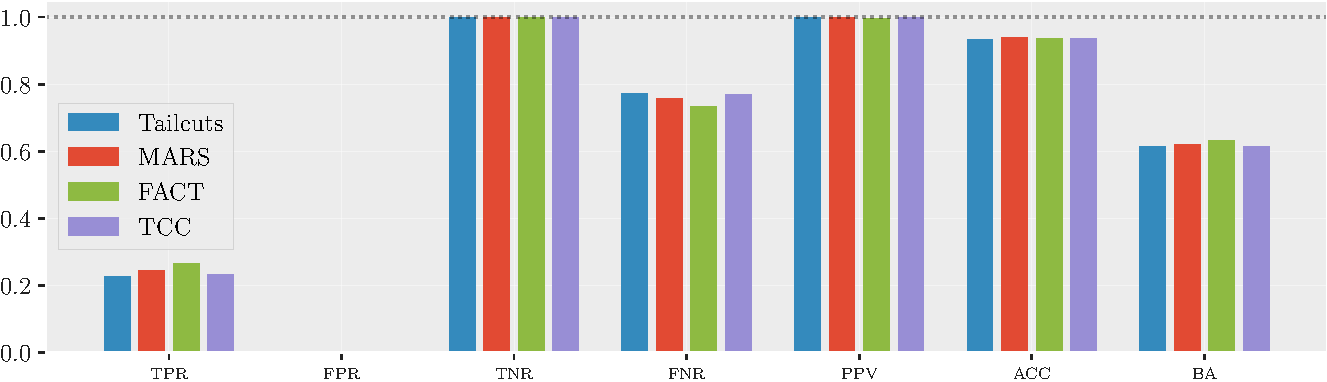
\includegraphics[width=\textwidth]{build/metrics_all.pdf}
    \caption{Bar plot visualizing the metrics for the selected settings of all four cleaning algorithms.
    \fact{} performs best out of all cleaning algorithms, followed by \mars{} and \tcc{}. The latter, however
    performs well \wrt the angular resolution, as shown in \autoref{fig:rel_angres} and can therefore be considered
    a viable alternative to \fact{}.}
    \label{fig:metrics_all}
\end{figure}
\chapter{Conclusions and Outlook}
\label{ch:conclusions}

In the scope of this work, the hyperparameters for each of the four currently (as of writing this thesis)
implemented cleaning algorithms were searched via a grid search. The resulting hyperparameters were then
probed \wrt a combined metric of the angular resolution and the efficiency. These results led to a subset
consisting of the best-performing hyperparameters for each cleaning algorithm. Furthermore, a comparison between the
optimized algorithms and the default algorithms, as well as a comparison between each respective
cleaner was performed.

Most of the data (pre-)processing in this work was done with \gls{cta}'s open-source low-level data processing pipeline
software \ctapipe{}, version \texttt{0.15.1}. The data used was PROD5 \gls{mc} simulations consisting of
\(\num{1.3}\)\,M telescope events (\sim\(\num{620}\)\,k array events) throughout \(987\) runs. The data
was processed from raw \texttt{simtel} data (\rzero) up to cleaned (\dloa) and parametrized (\dlob) levels
for the metrics as well as reconstructed (\dlt) data for the efficiency and angular resolution.
Further high-level processing was done with this works pipeline as described in \autoref{sec:pipeline}.

The four implemented cleaning algorithms can be roughly categorized into time-based (\fact{} and \tcc) and non-time-based
algorithms (\tailcuts{} and \mars{}). While the non-time-based algorithms only take thresholds of the photon count of each pixel
into account, the time-based algorithms also set limits on the arrival time of each pixel. This allows
for a lower core threshold \(Q_c\) for the photon count per pixel, which in turn can lead to better
results in the cleaning process. A good cleaning not only reduces data size---as a majority of the
pixels in the image are made up by \gls{nsb}---but it also allows for a better parameterization and in turn
a better reconstruction of the events.

The main results of this thesis are the hyperparameters for the cleaning algorithms.
Due to the long runtimes of the grid searches and the time limitation of this thesis, however, the hyperparameters
for cleaning algorithms were only optimized for \glspl{mst}. The optimal hyperparameters of each cleaning algorithm for
the \glspl{mst} are listed in \autoref{tab:best_parameters}. A further grid search with only \gls{lst}
data would be necessary to find the remaining core and boundary thresholds \(Q_c\) and \(Q_b\) as well
as the time limits for the \gls{lst} data.

The comparison of the performance of the optimized algorithms with the default algorithms has shown that
the optimized algorithms performed better than the default algorithms \wrt the angular resolution. This
means that the found hyperparameters could help with origin reconstructions. When looking at the metrics,
however, only \tcc{} really improved, while \fact{} even performed worse than its default implementation.
The reason might be, that the higher core threshold \(Q_c\)---compared to the default value---would
select fewer pixels. Additionally, a comparison between the optimized algorithms themselves was performed. This led to \fact{}
being the best performing algorithm overall \wrt the metrics, with only a slight advantage over the
other algorithms, however.

All in all, one can say, that the hyperparameters determined at a higher efficiency return better results,
albeit resulting in a higher angular resolution. This is due to the fact that a higher efficiency means
that more events got reconstructed and therefore better overall statistics. Nevertheless, further analysis
and a broader grid search might be necessary to find better hyperparameters
and therefore better the performance of all algorithms. This will also be necessary for the \gls{lst} data.



\backmatter
\printbibliography

\appendix
% Hier beginnt der Anhang, nummeriert in lateinischen Buchstaben
\chapter{Appendix}

\section{Configurations for \ctapipe{}}
\label{ap:aict_config}

The listings below show the contents of the default configuration files used for \ctapipe{}
with for each cleaning algorithm respectively.

\begin{description}
    \item \textbf{\tailcuts{}}:\medskip
    \begin{spacing}{0.5}
        \begin{mdframed}[backgroundcolor=codebg, hidealllines=true, leftmargin=0cm,rightmargin=0cm, skipabove=0pt, innerleftmargin=0,innerrightmargin=0,]
        \lstinputlisting[basicstyle=\lstsansserif, language=yaml]{./configs/tailcuts_clean_config.yml}
        \end{mdframed}
    \end{spacing}

    \item \textbf{\mars{}}:\medskip
    \begin{spacing}{0.5}
        \begin{mdframed}[backgroundcolor=codebg, hidealllines=true, leftmargin=0cm,rightmargin=0cm, skipabove=0pt, innerleftmargin=0,innerrightmargin=0,]
        \lstinputlisting[basicstyle=\lstsansserif, language=yaml]{./configs/mars_cleaning_1st_pass_config.yml}
        \end{mdframed}
    \end{spacing}

    \item \textbf{\fact{}}:\medskip
    \begin{spacing}{0.5}
        \begin{mdframed}[backgroundcolor=codebg, hidealllines=true, leftmargin=0cm,rightmargin=0cm, skipabove=0pt, innerleftmargin=0,innerrightmargin=0,]
        \lstinputlisting[basicstyle=\lstsansserif, language=yaml]{./configs/fact_image_cleaning_config.yml}
        \end{mdframed}
    \end{spacing}

    \item \textbf{\tcc{}}:\medskip
    \begin{spacing}{0.5}
        \begin{mdframed}[backgroundcolor=codebg, hidealllines=true, leftmargin=0cm,rightmargin=0cm, skipabove=0pt, innerleftmargin=0,innerrightmargin=0,]
        \lstinputlisting[basicstyle=\lstsansserif, language=yaml]{./configs/time_constrained_cleaning_config.yml}
        \end{mdframed}
    \end{spacing}
\end{description}

The following listing shows the contents of the \texttt{prod5b\_lapalma\_alpha.yml} configuration file,
which is used to set the allowed telescope IDs for \ctapipe{}\texttt{-process}.
\begin{spacing}{0.5}
    \begin{mdframed}[backgroundcolor=codebg, hidealllines=true, leftmargin=0cm,rightmargin=0cm, skipabove=0pt, innerleftmargin=0,innerrightmargin=0,]
    \lstinputlisting[basicstyle=\lstsansserif, language=yaml]{./configs/prod5b_lapalma_alpha.yml}
    \end{mdframed}
\end{spacing}


\newgeometry{margin=3cm, bottom=5cm}
\chapter{Acknowledgments}

\restoregeometry

\cleardoublepage
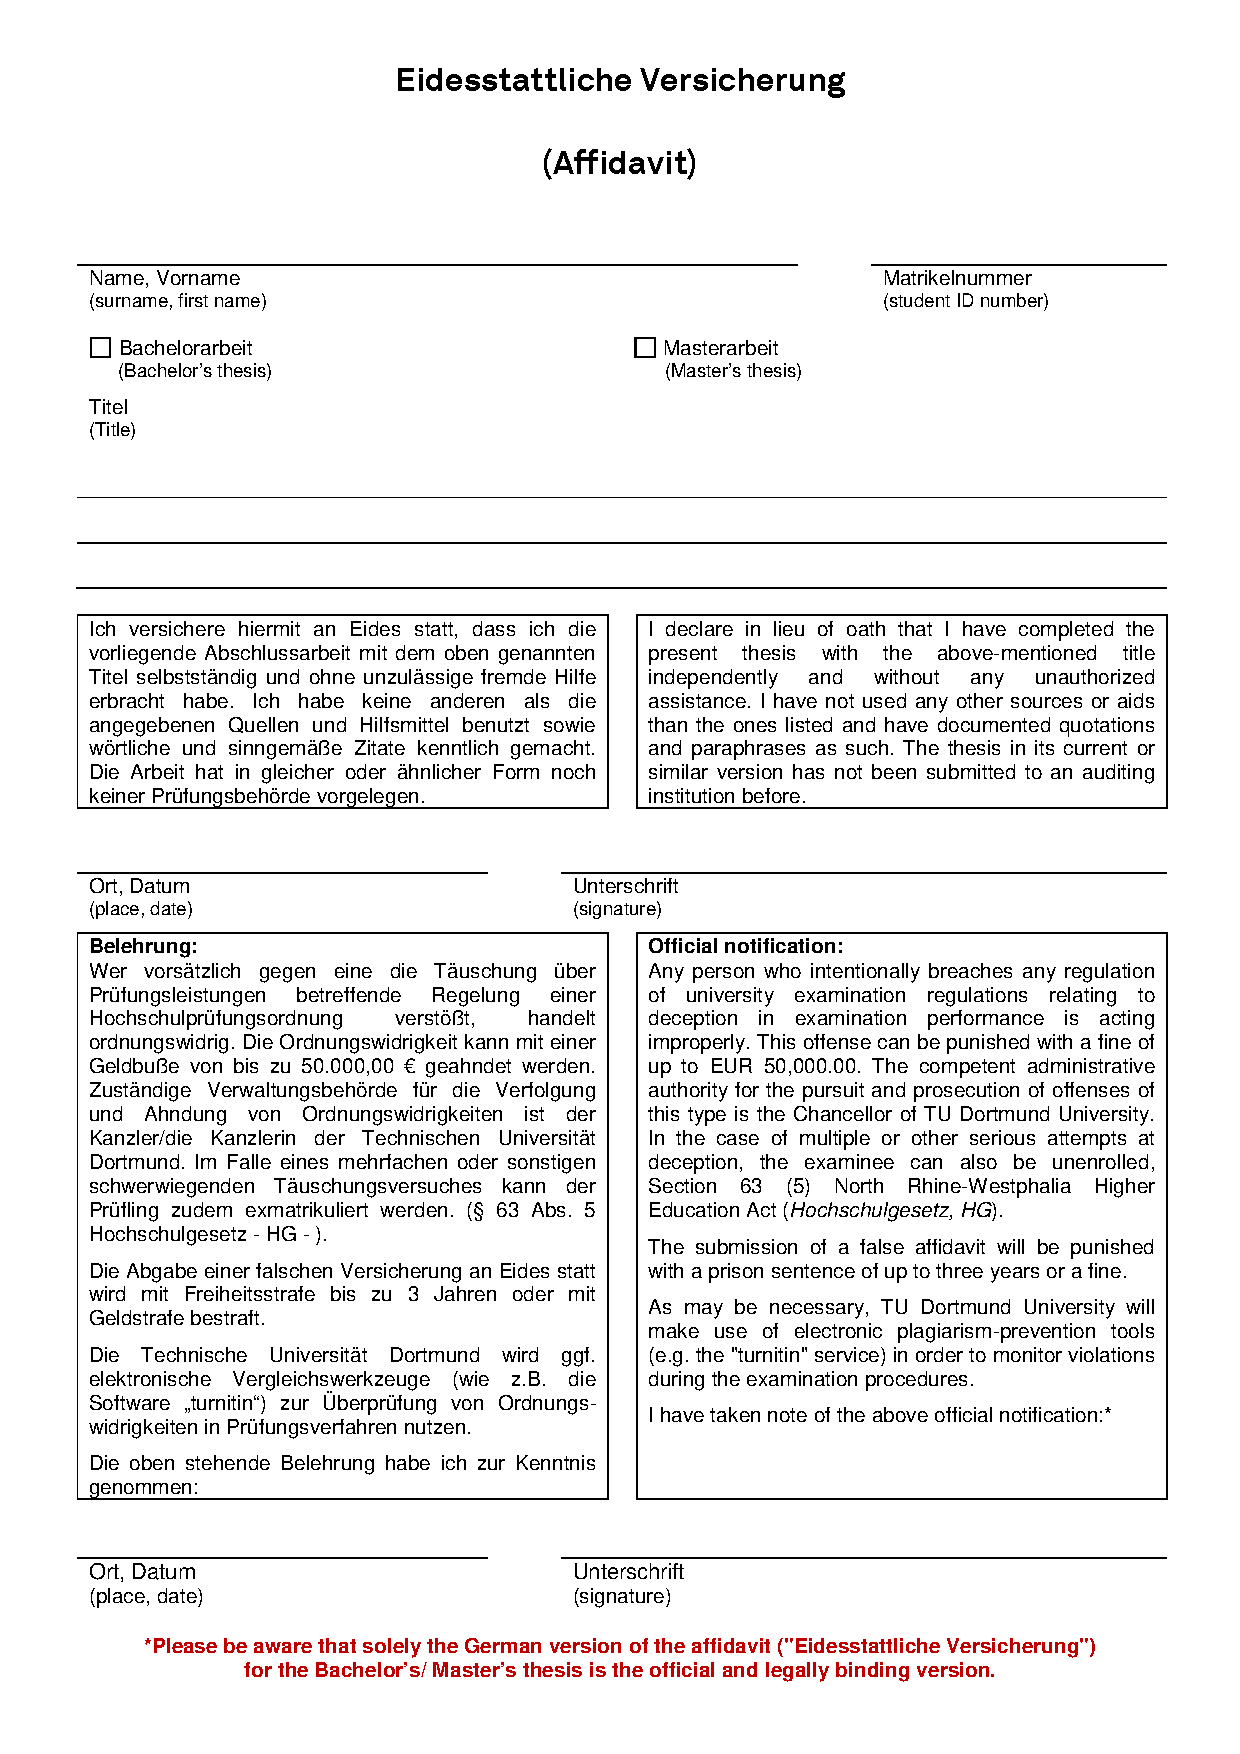
\includepdf{content/affidavit.pdf}

\end{document}
